\documentclass{pracamgr}
\usepackage{polski}
\usepackage{indentfirst}
\usepackage{parskip}
\usepackage{graphicx}
\usepackage{tabularx}
\usepackage{setspace}
\usepackage{listings}
\usepackage{hyphenat}
\usepackage{mdwlist}
\usepackage{fontspec}
\usepackage{xunicode}
\usepackage{xltxtra}
\usepackage{xeCJK}
\usepackage[hyphens]{url}
\usepackage{booktabs}
\usepackage{tocloft}

\hyphenation{MySQL jQuery Google In-sti-tute En-cyc-lo-pae-dia En-cyc-lo-pæ-dia Pre-pro-cessor}

% USTAWIENIA PAKIETÓW
\setmainfont[Mapping=tex-text,Bold=Charis SIL Bold,Scale=1.1]{Gentium}
\setsansfont[Mapping=tex-text]{Calibri}
\setmonofont[Scale=0.8]{DejaVu Sans Mono}
\setCJKmainfont[Scale=0.8]{Sazanami Mincho}
\lstset{tabsize=4, basicstyle=\ttfamily, columns=fixed, showstringspaces=false, extendedchars=true, breaklines=true,
	showtabs=false, showspaces=false, showstringspaces=false}
\graphicspath{{./screeny/}}

% USTAWIENIA KLASY PRACAMGR
\author{Krzysztof Dudzik}
\nralbumu{248349}
\title{Aplikacja wspomagająca tworzenie i~edycję haseł w~polskim Wikisłowniku}
\tytulang{An application supporting article creation and edition for the Polish Wiktionary}
\kierunek{Informatyka}
\opiekun{dr. hab. Jerzego Tyszkiewicza, prof. UW\\Instytut Informatyki\\}
\date{2011}
\dziedzina{11.3 Informatyka\\}
\klasyfikacja{H. Information Systems\\H.5. Information Interfaces and Presentation\\H.5.3. Group and Organization Interfaces}
\keywords{Wikisłownik, Fundacja Wikimedia, MediaWiki, wiki, edytor, API, JavaScript, jQuery, interfejs użytkownika, społeczność internetowa, open source}

% USTAWIENIA TYPOGRAFII
\setkeys{Gin}{width=0.9\textwidth}
\setlength{\fboxsep}{0pt}
\setlength{\fboxrule}{0.2pt}
\setlength{\parskip}{1.2ex plus 0.5ex minus 0.2ex}
\setlength{\parindent}{3ex}
\frenchspacing
\brokenpenalty=1000
\clubpenalty=1000
\widowpenalty=1000
\linespread{1.5}

% MAKRA I DEFINICJE

\let\kod\lstinline
\renewcommand*{\figurename}{Ilustracja}
\renewcommand*{\listfigurename}{Spis ilustracji}
\renewcommand{\cftpartdotsep}{\cftdotsep}
\renewcommand{\cftchapdotsep}{\cftdotsep}
\newcommand{\spacer}{
	\begin{center}
		\textasteriskcentered
	\end{center}
}
\newcommand{\solidrule}{
	\begin{center}
		\line(1,0){250}
	\end{center}
}
\newenvironment{illustration}[0]{
	\begin{figure}[ht]
	\begin{center}
}{
	\end{center}
	\end{figure}
}
\newenvironment{opis}[0]{
	\begin{basedescript}{\desclabelstyle{\pushlabel}\desclabelwidth{6em}}\setlength{\itemsep}{-2mm}
}{
	\end{basedescript}
}

% POCZĄTEK DOKUMENTU
\begin{document}
\maketitle

\begin{abstract}
  Tematem pracy jest aplikacja służąca do ułatwienia pracy autorów haseł w~polskim Wikisłowniku. Jej funkcje mają w~maksymalny możliwy sposób ułatwić tworzenie i~edytowanie haseł osobom bez wiedzy informatycznej i~technicznej, a~także automatyzować możliwie wiele rutynowych czynności wykonywanych przy redagowaniu hasła, jak tworzenie łącz do haseł powiązanych, zautomatyzowane szukanie przykładów użycia, wystąpień w~związkach frazeologicznych, wyrazów bliskoznacznych, innych słów, którą formę gramatyczną mogłoby stanowić hasło~itp. Dodatkowo aplikacja może przejąć część funkcji realizowanych obecnie za~pomocą botów.
\end{abstract}

\tableofcontents


\chapter{Wprowadzenie}
Żyjemy w~czasach, w~których nieustannie zmienia się sposób wyszukiwania informacji przez przeciętnego człowieka. Z~roku na rok coraz mniejszą rolę odgrywają papierowe kompendia takie jak encyklopedie i~słowniki, stopniowo przybierają natomiast na znaczeniu elektroniczne bazy wiedzy -- szczególnie zaś internetowe zbiory danych. Przyczyny tego stanu rzeczy są oczywiste: chodzi przede wszystkim o~wygodę korzystania ze~stron internetowych. Brak możliwości wyszukiwania w~obrębie ogromnych ilości danych powoduje, że encyklopedie i~słowniki w~postaci książek stają się o~wiele mniej atrakcyjne dla kogoś, kto chce zdobyć nowe informacje.

Wszechobecny dostęp do internetu sprawia, że to właśnie w~sieci WWW powstają najbardziej popularne bazy ludzkie wiedzy. Nie ma chyba internautów, którzy nie korzystaliby, rzadziej lub częściej, z~Wikipedii -- internetowej encyklopedii pisanej przez ochotników. Właśnie fakt, że encyklopedia ta współtworzona jest przez amatorów, stanowi o~jej wyjątkowym charakterze, który zostanie w~tej pracy pokrótce opisany. Wikipedia stale utrzymuje się w~pierwszej dziesiątce najczęściej odwiedzanych stron, a~pod wieloma względami jest to dziś najlepsza istniejąca encyklopedia. Przed kilkoma laty głośne było porównanie jej z~prestiżową \emph{Encyclopædia Britannica} -- okazało się, że różnice w~poziomie merytorycznym są niewielkie.

O~ile przewrót w~kategorii encyklopedii właściwie już się dokonał, nieco inaczej wygląda rywalizacja słowników. Oczywiście wyraźnie widać, że i~tu papierowe edycje są coraz mniej popularne. Różnice uwidaczniają się, gdy przeanalizowana zostanie sytuacja słowników internetowych. Tak zwany siostrzany projekt Wikipedii, Wikisłownik, nie dominuje wśród konkurencji -- zarówno na świecie, jak i~w~Polsce. Przyczyny tego stanu rzeczy są złożone. Autor postanowił skupić się na kilku zagadnieniach, uwidaczniających się w~polskojęzycznej wersji Wikisłownika. W~tym celu konieczne było zbadanie społeczności zaangażowanej w~tworzenie tego projektu. Jego efektem było wykonanie prac programistycznych, których opis stanowi główną część niniejszego opracowania.

W~przypadku wszystkich projektów opartych na silniku programistycznym MediaWiki istotną barierą rozwoju jest sama technologia. Każdy ochotnik ma możliwość uczestniczenia w~rozwoju portalu, wiąże się to jednak z~koniecznością przystosowania się do wymagań stawianych przez oprogramowanie. Edytowanie haseł w~internetowej encyklopedii czy słowniku jest praktycznie niemożliwe dla osoby bez wcześniejszego przygotowania lub znacznej wiedzy techniczno\dywiz{}informatycznej. Oprogramowanie MediaWiki oparte jest bowiem na tzw. wikikodzie (także: wikitekst, wikiskładnia), czyli języku opisu struktury i~wyglądu strony internetowej -- prostszym niż HTML, jednak wciąż nieintuicyjnym dla kogoś, kto nie miał wcześniej do czynienia z~tego typu edytorami. Dlatego wielu potencjalnych współautorów zniechęca się do projektu już przy pierwszej próbie poprawy artykułu.

Aby zmienić tę sytuację, przygotowany został nowy edytor, dostosowany specjalnie do potrzeb polskiego Wikisłownika. Aplikacja pozwala na o~wiele prostsze tworzenie nowych i~zmienianie starych haseł niż poprzednia, standardowa. Dzięki użyciu jej jako domyślnej w~projekcie popularyzacja edytowania Wikisłownika wśród fachowców w~dziedzinach lingwistycznych okaże się łatwiejsze -- zniknie podstawowa bariera, jaką jest konieczność dostosowania się do skomplikowanych technicznych wymagań stawianych przez użyte oprogramowanie. Dodatkowo nowa aplikacja umożliwia zaawansowaną automatyzację tworzenia hasła. Wiele z~czynności zintegrowanych z~nowym edytorem do tej pory wymagało mozolnych poszukiwań w~artykułach Wikisłownika oraz innych projektach. Dzięki użyciu API udostępnianego przez serwisy Fundacji Wikimedia skomplikowane przeszukiwanie tysięcy stron udało się sprowadzić do kilku kliknięć.

W~dalszej części pracy opisany został proces tworzenia tego edytora. Pierwszy rozdział charakteryzuje pokrótce sam Wikisłownik, jak i~pokrewne projekty oraz oprogramowanie w~nich użyte. Następnie opisano społecznościowe aspekty tworzenia tego typu aplikacji ze szczególnym uwzględnieniem koncepcji \emph{wiki}. Ostatni rozdział wyczerpująco przedstawia szczegóły projektowe i~implementacyjne aplikacji.


\chapter{Wikisłownik}
Rozdział ten stanowi charakterystykę Wikisłownika -- sieciowego słownika opartego na oprogramowaniu MediaWiki. Wikisłownik jest jednym z~największych i~najpopularniejszych słowników dostępnych w~polskim internecie. W~kolejnych sekcjach projekt ten został opisany na różnych poziomach szczegółowości. Omówiono zarówno oprogramowanie, na jakim bazuje słownik, jak i~swego rodzaju ,,ekosystem'', w~którym znajduje on swoje miejsce.

\section{Projekty Fundacji Wikimedia}
Podmiotem odpowiedzialnym m.in. za rozwój Wikisłownika jest Wikimedia Foundation Inc. (opisywana dalej jako ,,Fundacja'') -- organizacja non\dywiz{}profit mająca siedzibę w~San Francisco w~Stanach Zjednoczonych, istniejąca od 2003 roku. Jak informuje strona internetowa polskiego partnera Fundacji, Stowarzyszenia Wikimedia Polska, \emph{celem fundacji jest sprzyjanie tworzeniu i~rozwojowi projektów o~otwartej treści opartych na technologii WikiWiki oraz dostarczanie społeczności internetowej pełnej zawartości wymienionych projektów za darmo i~bez zamieszczania reklam}~\cite{wm:pl}. Doskonale znaną, sztandarową inicjatywą Fundacji jest Wikipedia (\url{http://www.wikipedia.org}) -- największa obecnie encyklopedia internetowa, dostępna w~281~językach (stan z~sierpnia 2011 roku) i~zawierająca ponad 19~milionów haseł, w~tym ponad 3,7~miliona w~największej, angielskojęzycznej\footnote{Oficjalnie w~projektach Fundacji używane są określenia typu \emph{angielskojęzyczny}, \emph{polskojęzyczny}. Choć w~przypadku wersji polskojęzycznej znakomita większość uczestników projektów pochodzi z~Polski, nie jest to regułą dla innych edycji. W~dalszej części pracy przyjęto uproszczenie polegające na tym, że określenia typu \emph{polska Wikipedia}, \emph{angielski Wikisłownik} traktowane są jako tożsame z~określeniami używającymi sformułowań z~cząstką \emph{-języczny}.} edycji \cite{wiki:list}. Mimo częstej krytyki tego przedsięwzięcia faktem jest, że Wikipedia jest miejscem, z~którego miliony osób korzystają, by pozyskać informacje z~najróżniejszych dziedzin. Obecny stan rzeczy możliwy jest dzięki pracy wielkiej liczby wolontariuszy tworzących artykuły bez wynagrodzenia.

\begin{illustration}
	\fbox{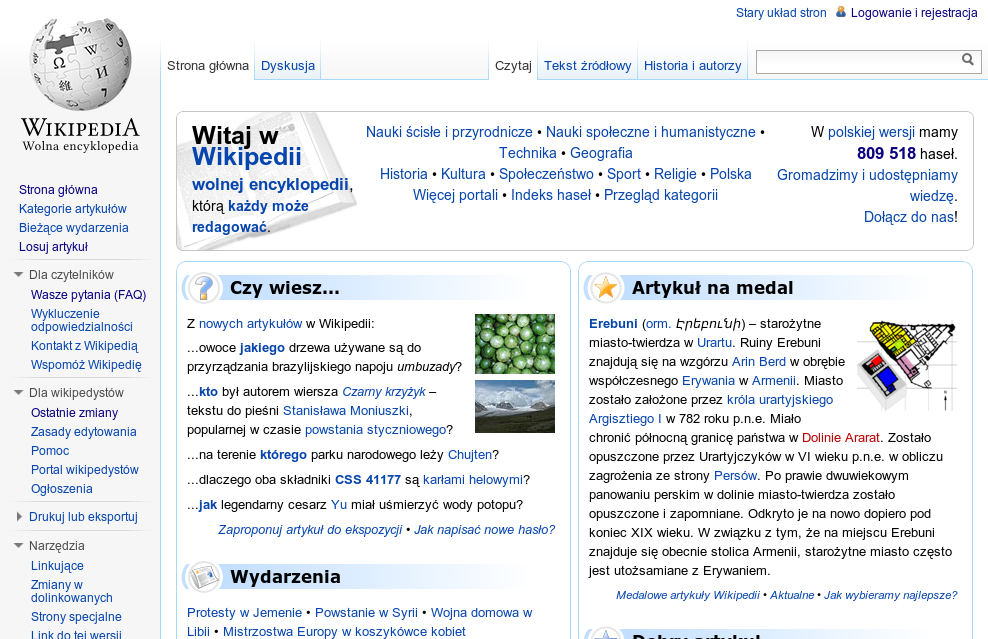
\includegraphics{plwikipedia}}
	\caption{Polska edycja Wikipedii}
\end{illustration}

Wikipedia jest najbardziej znanym, ale nie jedynym projektem pod opieką Fundacji. Pozostałe to tzw. ,,projekty siostrzane'', w~szczególny sposób uwzględniane również przy tworzeniu haseł w~encyklopedii. Oto lista wspieranych przez Fundację wielojęzycznych inicjatyw~\cite{wm:main}:
\begin{itemize}
	\item Wikisłownik (ang. \emph{Wiktionary}) -- wielojęzyczny słownik internetowy, będący głównym przedmiotem niniejszej pracy,
	\item Wikicytaty (ang. \emph{Wikiquotes}) -- zbiór cytatów autorstwa znanych osób, z~filmów i~książek, przysłów i~porzekadeł,
	\item Wikibooks -- serwis z~,,otwartymi'' (opartymi na wolnej licencji) podręcznikami,
	\item Wikiźródła (ang. \emph{Wikisource}) -- zbiór dokumentów źródłowych w~wersjach oryginalnych i~tłumaczonych, nieograniczonych prawem autorskim,
	\item Wikinews -- otwarty serwis informacyjny,
	\item Wikiversity -- materiały edukacyjne i~naukowe,
	\item Wikispecies -- katalog gatunków organizmów żywych,
	\item MediaWiki -- nadzór nad tworzeniem i~rozpowszechnianiem oprogramowania MediaWiki (p.~sekcja~\ref{sec:mw}),
	\item Meta\dywiz{}Wiki -- projekt ułatwiający koordynację wszystkich pozostałych.
	\item Wikimedia Commons -- repozytorium mediów (zdjęć, grafik, filmów) dostępnych na wolnej licencji, z~którego korzystają pozostałe projekty Wikimedia,
	\item Wikimedia Incubator -- metaprojekt umożliwiający tworzenie nowych inicjatyw wspieranych przez Fundację.
\end{itemize}
Wszystkie projekty łączy sposób ich powstawania -- możliwość edycji dostępna jest praktycznie dla każdego internauty. Nie dotyczy to co~prawda kilku krajów, w~których projekty Fundacji zablokowane są w~ramach cenzury internetu, jednak ogromna większość osób dysponujących łączem internetowym ma szansę stać się jednymi spośród współautorów haseł.

Drugą cechą wspólną są wolne licencje, na których udostępniana jest zawartość wszystkich serwisów. Po reformie w~czerwcu 2009~roku treść Wikipedii i~projektów siostrzanych dostępna jest nie tylko na licencji GNU FDL (Free Documentation License), ale także na kompatybilnej z~nią CC\dywiz{}BY\dywiz{}SA 3.0 (Creative Commons Attribution\dywiz{}ShareAlike / Uznanie Autorstwa -- Na Tych Samych Warunkach)~\cite{wiki:license}. Oznacza to, że można ją dowolnie wykorzystywać we~własnych dziełach pod warunkiem podania oryginalnych autorów i~zachowania pierwotnej licencji.

\section{Oprogramowanie MediaWiki}
\label{sec:mw}
Sama działalność wolontariacka redaktorów projektów Wikimedia nie wystarczyłaby do stworzenia serwisów internetowych o~obecnych kształtach. Konieczne jest oczywiście również zapewnienie oprogramowania, które umożliwi płynną współpracę przy tworzeniu haseł. Tym oprogramowaniem jest wolna platforma MediaWiki tworzona zgodnie z~zasadami \emph{open source}. System MediaWiki napisany jest w~języku PHP i~obsługuje kilka popularnych baz danych (w~przypadku projektów Wikimedia jest to MySQL). Dla inicjatyw Wikimedia stanowi szkielet programistyczny od samego ich początku, a~od 2002~roku stale się rozwija. W~czerwcu 2011~roku wersją używaną w~projektach było MediaWiki~1.17.

System MediaWiki używany jest nie tylko w~projektach wspieranych przez Fundację, ale także w~tysiącach innych, mniejszych lub większych, co jest możliwe dzięki wysokiemu stopniowi konfigurowalności i~dużej liczbie dostępnych rozszerzeń. Są to w~dużej mierze serwisy o~podobnym charakterze, umożliwiające swobodną wymianę informacji na dowolny temat. MediaWiki bywa także używane w~firmowych intranetach i~wszędzie tam, gdzie zachodzi potrzeba udostępnienia materiałów do edycji dużej liczbie użytkowników.

\subsection{Edytowanie i~wikitekst}
Strony w~projektach opartych na platformie MediaWiki na~ogół nie mogą być czystym tekstem, pozbawionym formatowania. Przykładowo hasła w~encyklopedii muszą zachowywać określoną strukturę -- występuje więc podział na sekcje, ilustracje, różne rodzaje formatowania (kursywa, wytłuszczenie), przypisy czy powtarzalne fragmenty. Szczególnie istotnym elementem są linki pomiędzy poszczególnymi artykułami, wyróżniające projekty Fundacji na tle ich papierowych, ale też elektronicznych konkurentów. Odnośniki pozwalają błyskawicznie przemieszczać się między hasłami, by w~ten sposób uzyskiwać kolejne informacje wspomagające przyswajanie wiedzy.

Linki i~formatowanie na stronach internetowych tworzone są za pomocą elementów języka HTML lub XHTML. O~ile języki te są proste w~obsłudze dla specjalisty informatyka, to laik nie jest w~stanie tworzyć za ich pomocą stron bez uprzedniego dłuższego przygotowania. Aby umożliwić bezproblemową edycję stron internetowych osobom bez wykształcenia informatycznego, programiści MediaWiki zaprojektowali tzw. wikitekst~\cite{mw:help} -- uproszczony język opisu stron, pozwalający na realizację wymienionych elementów. Porównanie niektórych z~nich znajduje się w~tabeli~\ref{tab:html-wiki}.

\begin{table}[h]
\begin{center}
\footnotesize{
	\begin{tabularx}{\textwidth}{ lXX }
		\toprule & \textbf{Wikitekst} & \textbf{XHTML} \\
		\toprule Kursywa & \texttt{''Tekst''} & \texttt{<em>Tekst</em>} \\
		\midrule Wytłuszczenie & \texttt{'''Tekst'''} & \texttt{<strong>Tekst</strong>} \\
		\midrule Nagłówek & \texttt{== Nagłówek ==} & \texttt{<h2>Nagłówek</h2>} \\
		 & \texttt{=== Nagłówek ===} & \texttt{<h3>Nagłówek</h3>} \\
		\midrule Odnośnik wewnętrzny & \texttt{[[Strona]]} & \texttt{<a href="/wiki/Strona">Strona</a>} \\
		 & \texttt{[[Strona|strony]]} & \texttt{<a href="/wiki/Strona">strony</a>} \\
		\midrule Odnośnik zewnętrzny & \texttt{[http://www.google.com Google]}
		 & \texttt{<a href="http://www.google.com">\newline Google</a>} \\
		\midrule Obraz & \texttt{[[Plik:Przykład.png|thumb|Podpis]]}
		 & \texttt{<img src=".../Przykład.png"/><br/>\newline <div class="caption">Podpis</div>} \\
		\midrule Podział na akapity & \texttt{Pierwszy akapit \newline \newline Drugi akapit}
		 & \texttt{<p>Pierwszy akapit</p>\newline <p>Drugi akapit</p>} \\
		\midrule Lista nienumerowana & \texttt{* Element\newline * Element\newline * Element}
		 & \texttt{<ul>\newline <li>Element</li>\newline <li>Element</li>\newline <li>Element</li>\newline </ul>}\\
		\midrule Lista numerowana & \texttt{\# Element\newline \# Element\newline \# Element}
		 & \texttt{<ol>\newline <li>Element</li>\newline <li>Element</li>\newline <li>Element</li>\newline </ol>}\\
		\bottomrule
	\end{tabularx}
}
\caption{Porównanie HTML i wikitekstu}
\label{tab:html-wiki}
\end{center}
\end{table}

Łatwo można zauważyć, że używanie wikitekstu jest o~wiele prostsze niż nauka języka XHTML. Jeśli zachodzi potrzeba zaawansowanego formatowania, możliwe jest także użycie znaczników XHTML. W~przypadku standardowego formatowania jest to jednak niewskazane ze względu na dobro niedoświadczonych edytorów.

Bardzo istotnym elementem wikitekstu są szablony -- predefiniowane fragmenty kodu z~opcjonalnymi parametrami. Szablony można uznać za odpowiednik procedur/funkcji w~językach programowania. W~projektach opartych na MediaWiki szablony pełnią przede wszystkim dwie główne funkcje:
\begin{itemize}
	\item upraszczają kod -- pozwalają np. na zastąpienie skomplikowanego kodu XHTML (a~także jeszcze bardziej złożonych funkcji parsera MediaWiki) krótkim wywołaniem szablonu,
	\item standaryzują strony -- często wykorzystywane fragmenty wywoływane są zawsze w~dokładnie ten sam sposób.
\end{itemize}
We~wszystkich większych projektach Fundacji szablony są bardzo często wykorzystywane. Przy tym stanowią duże ułatwienie dla technicznie zaawansowanych autorów, którzy wspomagają się przy tworzeniu haseł dodatkowymi technologiami. Na używaniu szablonów korzystają przede wszystkim boty, czyli programy dokonujące edycji samodzielnie po uprzednim przygotowaniu lub pod stałą opieką programisty. W~większości projektów przyjęte jest, że każdy bot ma własne konto użytkownika, nie używa natomiast konta swojego ,,właściciela''. Dzięki botom możliwe jest np. masowe tworzenie haseł w~Wikipedii na ściśle określony temat, jeśli istnieje dobre źródło w~formie czytelnej dla komputera (takich jak opisy asteroid czy wszystkich miejscowości lub jednostek administracyjnych w~danym kraju). Innym ich zastosowaniem jest automatycznie uzupełnianie tzw. interwiki -- czyli odnośników pomiędzy poszczególnymi wersjami językowymi tego samego hasła.

Szablony mogą być wykorzystywane w~prosty sposób nawet przez początkujących użytkowników -- aby wywołać szablon, wystarczy wpisać jego nazwę
 pomiędzy podwójnymi nawiasami klamrowymi (\kod@{{Nazwa szablonu}}@ lub \kod@{{Nazwa szablonu|parametr=abc}}@). W~polskim Wikisłowniku szablony pełnią szczególną rolę -- i~to m.in. dzięki ich szerokiemu zastosowaniu w~projekcie zrodził się pomysł na niniejszą pracę. Szczegóły tego zagadnienia zostaną przedstawione w~sekcji~\ref{sec:plwikt}.

\section{Wiktionary -- Wikisłownik}
\begin{illustration}
	\fbox{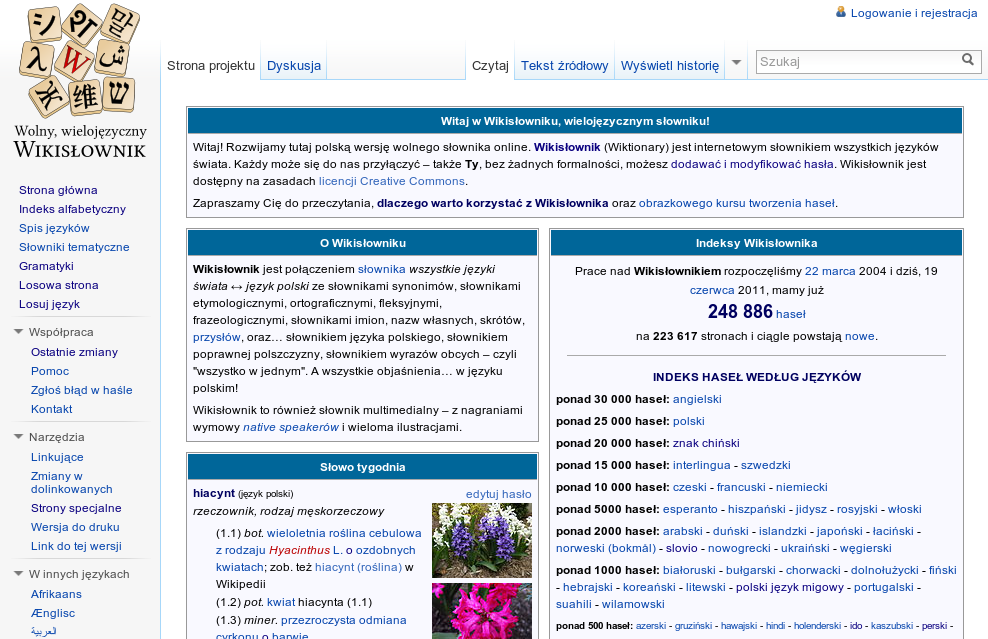
\includegraphics{plwikt}}
	\caption{Polska edycja Wikisłownika}
\end{illustration}
Jednym z~największych projektów siostrzanych Wikipedii jest Wikisłownik, w~wersji angielskiej (i~wielu innych) noszący nazwę \emph{Wiktionary} (\url{http://www.wiktionary.org}). Ten słownik internetowy nie rozwinął się jeszcze tak prężnie jak encyklopedia, zwłaszcza jeśli chodzi o~polską edycję. Jest dziś jednak jednym z~największych słowników w~sieci, a~w~pewnych zastosowaniach stanowi najlepszy wybór. Dużą zaletą Wikisłownika jest jego wielojęzyczność -- w~tym samym serwisie znaleźć można hasła w~ponad~250~językach. W~przypadku niektórych z~nich jest to praktycznie jedyny słownik internetowy lub nawet jedyny dostępny słownik w~ogóle. Przykładem może być polski Wikisłownik, który zawiera prawdopodobnie jedyny polski słownik języka hawajskiego czy największe słowniki języków suahili i~jidysz~\cite{wikt:dlaczego}.

Wspomniane zostało zastosowanie szablonów do standaryzacji kodu źródłowego i~struktury haseł. Trzeba jednak zaznaczyć, że dotyczy to wyłącznie haseł w~obrębie jednej wersji językowej Wikisłownika, są one bowiem niezależne od siebie i~od Fundacji. Wspólne dla wszystkich edycji jest jedynie oprogramowanie MediaWiki i~umiejscowienie na serwerach Fundacji pod adresem \kod|xxx.wiktionary.org|, gdzie zamiast \kod|xxx| wstawiany jest dwu- lub trzyliterowy skrót ISO języka (np. \url{pl.wiktionary.org} = język polski, \url{de.wiktionary.org} = język niemiecki, \url{sq.wiktionary.org} = język albański, \url{csb.wiktionary.org} = język kaszubski). Wszystkie kwestie organizacyjne w~obrębie wersji językowej ustalane są w~ramach dyskusji i~głosowań przez internetową społeczność. Głosowania służą także wyborowi administratorów projektu, czyli użytkowników mających dodatkowe uprawnienia, spośród których najważniejsze to usuwanie i~zabezpieczanie haseł oraz blokowanie użytkowników działających na szkodę projektu. W~lipcu 2011~roku w~angielskim Wikisłowniku działało aktywnie 76~administratorów~\cite{enwikt:admin}, zaś w~polskim -- 14~\cite{wikt:admin}. Dla porównania Wikipedia w~języku angielskim ma 1541~administratorów (niekoniecznie aktywnych), wersja polska natomiast 163~\cite{wiki:admin}.

Podobnie jak w~przypadku Wikipedii, hasła w~poszczególnych wersjach językowych Wikisłownika są łączone poprzez odnośniki interwiki, znajdujące się na dole lewego menu w~większości haseł. W~stosunku do encyklopedii występuje znacząca różnica w~sposobie funkcjonowania tych linków. Wikipedia poprzez interwiki łączy artykuły na ten sam temat, często różniące się tytułem (polski artykuł \emph{Kot domowy} odsyła do angielskiego \emph{Cat} czy niemieckiego \emph{Hauskatze}). W~Wikisłowniku mechanizm interwiki łączy zaś strony o~tym samym tytule, niezależnie od ich zawartości. Polskie hasło \emph{kot} zawiera więc łącza do haseł o~tytule \emph{kot} w~innych językach, które mogą, ale nie muszą zawierać m.in. objaśnienia polskiego znaczenia tego słowa. Z~tego względu łatwo jest odnaleźć brakujące informacje o~wybranym słowie w~danym języku, jeśli skorzysta się z~kilku edycji językowych Wikisłownika. Natomiast tłumaczenia tytułu hasła na inne języki znajdują się bezpośrednio w~treści artykułu, w~miejscu przeznaczonym dla takich informacji.

Choć poszczególne wersje Wikisłownika różnią się między sobą, wspólna jest struktura hasła na najogólniejszym poziomie. Każde hasło jest podzielone na sekcje nagłówkami 2.~stopnia (p.~tabela~\ref{tab:html-wiki}), podobnie jak w~innych projektach Fundacji. W~przypadku słownika sposób podziału artykułu został jasno sprecyzowany i~jest wspólny dla wszystkich edycji. W~każdej z~sekcji objaśniono znaczenie tytułowego hasła w~innym języku. Przykładowo hasło \emph{nie} w~większości wersji językowych ma sekcje objaśniające znaczenie m.in. w~języku polskim oraz języku niemieckim (\emph{nigdy}). Właśnie ta ogólna cecha struktury haseł pozwala na częściową automatyzację niektórych często wykonywanych w~trakcie edycji czynności.

Aplikacja opisana w~niniejszej pracy przeznaczona jest dla polskiej edycji Wikisłownika. Konieczne jest zatem scharakteryzowanie specyfiki tego projektu (p.~sekcja~\ref{sec:plwikt}). Ze~względu na odmienność poszczególnych wersji językowych prawdopodobnie w~innych nie będzie można wykorzystać wykorzystać aplikacji. Z~pewnością może ona być dla nich jednak bardzo przydatna -- duża część funkcji przez nią realizowanych może być używana niezależnie od specyfiki danej wersji, a~budowa aplikacji pozwoli na ich wyodrębnienie.

\section{Polska edycja Wikisłownika}
\label{sec:plwikt}
Wikisłownik w~języku polskim powstał 22~marca 2004~r.~\cite{wikt:home} i~jest dziś jedną z~najlepiej rozwiniętych edycji. Jeśli chodzi o~liczbę haseł, polska wersja zawiera ich ponad 230~000 i~znajduje się na 8.~miejscu (pierwsze trzy miejsca zajmują z~dużą przewagą edycje angielska, francuska i~chińska). Warto zwrócić jednak uwagę, że liczba artykułów nie musi odzwierciedlać ogólnego poziomu rozwoju danej edycji, a~przynajmniej w~o~wiele mniejszym stopniu niż w~Wikipedii. Automatyczne importowanie haseł słownikowych z~innych źródeł jest prostsze niż w~przypadku wpisów do~encyklopedii, a~hasła takie oczywiście nie wyróżniają się pozytywnie pod względem jakości. Wydaje się, że lepszym wskaźnikiem rozwoju są np. liczby aktywnych użytkowników lub administratorów. Tutaj polski Wikisłownik okazuje się wielokrotnie lepszy niż edycje litewska czy malajska, górujące nad nim pod względem liczby haseł~\cite{wikt:list}.

W~kolejnej podsekcji opisana została dokładnie struktura haseł w~polskim Wikisłowniku. Społeczność tego projektu scharakteryzowano natomiast w~sekcji~\ref{sec:plsoc}.

\subsection{Struktura hasła}
Jak wspomniano, wspólny dla wszystkich wersji językowych Wikisłownika jest podział na sekcje, odpowiadające poszczególnym językom. Polska edycja Wikisłownika jest bardzo dobrze ustrukturyzowana w~dalszym zakresie, co niekoniecznie jest regułą dla pozostałych edycji. Wynikiem tego jest jednolity wygląd hasła, który otrzymuje czytelnik, oraz jednolity kod widziany przez redaktora. Przykładowy artykuł z~jedną sekcją językową znajduje się na ilustracji~\ref{fig:plhaslo}.

\begin{illustration}
	\fbox{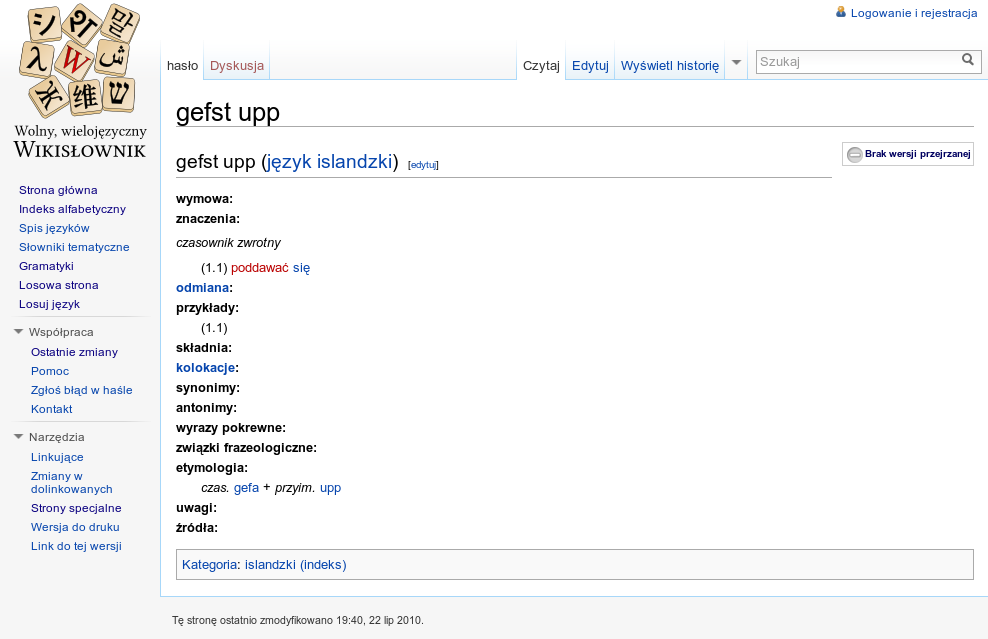
\includegraphics{plwikt-art}}
	\caption
		[Hasło w~polskim Wikisłowniku]
		{Hasło \emph{gefst upp} w~polskim Wikisłowniku (\protect\url{http://pl.wiktionary.org/wiki/gefst_upp})}
	\label{fig:plhaslo}
\end{illustration}

Na zrzucie ekranu widoczny jest układ sekcji typowy dla polskiego projektu. Z~małymi wyjątkami sekcje danego języka wyglądają tak samo we~wszystkich hasłach. To oznacza, że także w~innych opisanych wyrazach języka islandzkiego znaleźć można elementy: wymowa, znaczenia, odmiana, przykłady, składnia, kolokacje, synonimy, antonimy, wyrazy pokrewne, związki frazeologiczne, etymologia, uwagi, źródła. W~rzeczywistości jest to układ typowy dla znakomitej większości występujących w~Wikisłowniku języków~\cite{wikt:zasady}. Odstępstwa od tego szkieletu hasła są niewielkie i~zostaną przedstawione poniżej.

Ilustracja~\ref{fig:plhaslo-edit} przedstawia wygląd przykładowej strony po przejściu do trybu edycji, dostępnego dla każdego użytkownika (bez konieczności logowania). Widok ten prezentuje źródłowy wikikod hasła, dodatkowo edytor ma kilka ikon ułatwiających wstawianie często używanych elementów. W~kodzie tym widoczne są szablony definiujące tytuły poszczególnych elementów sekcji (nazywanych dalej \emph{podsekcjami}). Podział na sekcje i~podsekcje jest dość prosty do wykonania za pomocą programu komputerowego i~już sama ta procedura pozwala na znaczne zwiększenie przejrzystości w~nowym edytorze, opisanym w~rozdziale~\ref{chap:impl}.

\begin{illustration}
	\fbox{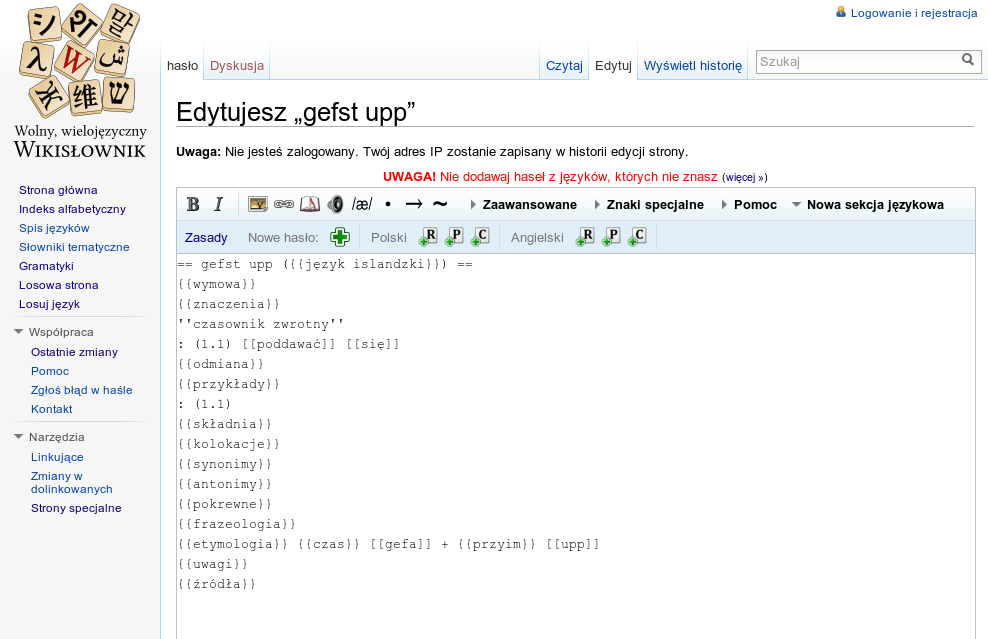
\includegraphics{plwikt-edit}}
	\caption
		[Edycja hasła w~polskim Wikisłowniku]
		{Edycja hasła \emph{gefst upp} w~polskim Wikisłowniku (\protect\url{http://pl.wiktionary.org/w/index.php?title=gefst_upp&action=edit})}
	\label{fig:plhaslo-edit}
\end{illustration}

Każda z~podsekcji w~hasłach ma ściśle określoną funkcję, dzięki której polski Wikisłownik jest jednolity. Poniżej zostały omówione wszystkie podsekcje występujące w~artykułach, w~jedynej przyjętej jako poprawną kolejności. Duża ich część pojawia się jedynie w~niektórych językach, dlatego choć lista podsekcji jest dość długa, to każde hasło będzie miało ich o~wiele mniej. Szablony podsekcji zebrane są na stronie \url{http://pl.wiktionary.org/wiki/Kategoria:Szablony_szablonów_haseł}.

\subsubsection{Podsekcje występujące w~hasłach polskiego Wikisłownika}
\label{wikt:subsections}
\begin{opis}
	\item[Szablon] \verb|{{zapis hieroglificzny}}|
	\item[Zawartość] Zapis hieroglificzny słowa w~języku staroegipskim, pokazany za~pomocą grafik PNG z~repozytorium Wikimedia Commons. Oznaczenie \kod|(1.1)| odnosi się do numeracji w~sekcji \emph{znaczenia}.
	\item[Języki] tylko staroegipski\footnote{Rubryka \emph{Języki} precyzuje, w~których sekcjach językowych występuje dana podsekcja. Oprócz zwykłych sekcji, odpowiadających danemu językowi, istnieją także nietypowe: \emph{użycie słowa obcego w~języku polskim} i~\emph{znak chiński}}.
	\item[Przykład]
		\begin{verbatim}
			{{zapis hieroglificzny}}
			: (1.1) [[Plik:Egyptian-Pr-cnḫ.PNG]];
			[[Plik:Egyptian-Pr-cnḫ2.PNG]];
			[[Plik:Egyptian-Pr-cnḫ3.PNG]]
		\end{verbatim}
\end{opis}
\spacer
\begin{opis}
	\item[Szablon] \verb|{{ortografie}}|
	\item[Zawartość] Inne sposoby zapisu tytułu hasła. Zazwyczaj chodzi o~alternatywną pisownię w~języku, do zapisu którego używane są dwa alfabety (np.\ serbski). Do prezentacji pisowni mogą być używane szablony wyświetlające dodatkowe informacje.
	\item[Języki] azerski, białoruski, dżuhuri, gagauski, krymskotatarski, ladino, mołdawski, serbski, slovio, tatarski, turkmeński, ujgurski
	\item[Przykład]
		\begin{verbatim}
			{{ortografie}} Мацедониа
		\end{verbatim}
\end{opis}
\spacer
\begin{opis}
	\item[Szablon] \verb|{{transliteracja}}|
	\item[Zawartość] Transliteracja słowa zapisanego w~obcym alfabecie na alfabet łaciński. \\ W~przeciwieństwie do transkrypcji transliteracja może być wykonywana automatycznie --- każda litera alfabetu obcego konwertowana jest na jeden lub więcej znaków w~alfabecie łacińskim. Obecnie często używany jest szablon \kod|{{translit}}|, który umożliwia automatyczną konwersję za pomocą JavaScriptu niektórych alfabetów podczas odczytywania strony.
	\item[Języki] abazyński, abchaski, adygejski, akadyjski, amharski, arabski, aramejski, assamski, awarski, baszkirski, beludżi, bengali, birmański, bułgarski, chakaski, czeczeński, czuwaski, dzongkha, erzja, gocki, gruziński, gudźarati, gyyz, hebrajski, hindi, inguski, inuktitut, jidysz, kannada, kaszmirski, kazachski, khmerski, kirgiski, komi, komi\dywiz{}jaźwiński, kri, kurdyjski, laotański, lezgiński, macedoński, malajalam, malediwski, marathi, maryjski, mongolski, nepalski, newarski, nowogrecki, orija, ormiański, osetyjski, paszto, pendżabski, perski, romski, rosyjski, sanskryt, sindhi, sorani, staro\dywiz{}cerkiewno\dywiz{}słowiański, starogrecki, staroormiański, sumeryjski, syngaleski, tabasarański, tadżycki, tajski, tamazight, tamilski, telugu, tybetański, ukraiński, urdu, zarfatit
	\item[Przykład]
		\begin{verbatim}
			{{transliteracja}} Moskva
		\end{verbatim}
\end{opis}
\spacer
\begin{opis}
	\item[Szablon] \verb|{{transkrypcja}}|
	\item[Zawartość] Transkrypcja słowa zapisanego w~obcym alfabecie na język polski, czyli przedstawienie go w~formie dającej informacje o~rzeczywistej wymowie
	\item[Języki] standardowo tylko staroegipski, podsekcja ta może być jednak dodawana w~wielu innych językach (przykład w~jidysz)
	\item[Przykład]
		\begin{verbatim}
			{{transkrypcja}}
			: (1.1-3) {{YIVO|{{lp}} khaver {{lm}} khaveyrim}}; polska: {{lp}}
			chawer {{lm}} chawejrim
			: (1.4) {{YIVO|{{lp}} khover {{lm}} khovers}}; polska: {{lp}}
			chower; {{lm}} chowers
		\end{verbatim}
\end{opis}
\spacer %http://pl.wiktionary.org/wiki/Kategoria:Szablony_szablon%C3%B3w_hase%C5%82
\begin{opis}
	\item[Szablon] \verb|{{czytania}}|
	\item[Zawartość] Wyjaśnienie możliwego wymawiania znaków kanji używanych w~języku japońskim. Występują dwa sposoby czytania: on'yomi i~kun'yomi. Do ich prezentacji używane są szablony \kod|{{on}}| i~\kod|{{kun}}|.
	\item[Języki] tylko japoński
	\item[Przykład]
		\begin{verbatim}
			{{czytania}} {{on}} ビ (bi); {{kun}} はな (hana)
		\end{verbatim}
\end{opis}
\spacer
\begin{opis}
	\item[Szablon] \verb|{{klucz}}|
	\item[Zawartość] Elementy, według których układane są słowniki języka chińskiego.
	\item[Języki] tylko znak chiński
	\item[Przykład]
		\begin{verbatim}
			{{klucz}} 157 足 + 6
		\end{verbatim}
\end{opis}
\spacer
\begin{opis}
	\item[Szablon] \verb|{{kreski}}|
	\item[Zawartość] Liczba kresek użytych do napisania danego znaku. Informacja służy m.in.\ do ułatwienia odnajdywania znaków w~papierowych słownikach.
	\item[Języki] znak chiński, koreański
	\item[Przykład]
		\begin{verbatim}
			{{kreski}} 13
		\end{verbatim}
\end{opis}
\spacer
\begin{opis}
	\item[Szablon] \verb|{{warianty}}|
	\item[Zawartość] Szablon powiększający znak chiński i~ewentualnie jego warianty. Szablon ten jest używany inaczej niż większość: nie odpowiada jedynie za wyświetlenie nagłówka, a~zawartość sekcji wstawiana jest jako parametr. Najczęściej w~parametrze pojawia się szablon \kod|{{zch-w}}|, odpowiadający za prezentację znaku.
	\item[Języki] tylko znak chiński
	\item[Przykład]
		\begin{verbatim}
			{{warianty|{{zch-w}}}}
		\end{verbatim}
\end{opis}
\spacer
\begin{opis}
	\item[Szablon] \verb|{{kolejność}}|
	\item[Zawartość] Kolejność stawiania kresek w~znaku chińskim, ilustrowana za pomocą grafiki dostępnej w~projekcie Wikimedia Commons. W~tej podsekcji używane są szablony \kod|{{zch-komiks}}|, \kod|{{zch-cienie}}| i~\kod|{{zch-animacja}}|, które ładują automatycznie grafiki o~nazwie odpowiadającej hasłu, jeśli te istnieją.
	\item[Języki] tylko znak chiński
	\item[Przykład]
		\begin{verbatim}
		{{kolejność}}
		{{zch-komiks}}
		\end{verbatim}
\end{opis}
\spacer
\begin{opis}
	\item[Szablon] \verb|{{wymowa}}|
	\item[Zawartość] Jedna z~kluczowych podsekcji we~wszystkich językach. Podawane są w~niej informacje na temat wymowy danego hasła, zarówno za pomocą alfabetów fonetycznych (jak np.\ IPA oraz alfabet słowiański), jak i~nagrań dźwiękowych umieszczonych w~Wikimedia Commons. Do opisywania wymowy stosowane są szablony \kod|{{IPA}}|, \kod|{{IPA2}}|, \kod|{{IPA3}}|, \kod|{{IPA4}}|. Wymowa słów polskich dodawana jest automatycznie przez bota uruchomionego przez jednego z~administratorów Wikisłownika. Bot ten jest skomplikowanym programem napisanym w~Javie~\cite{wikt:olafbot}, generującym wymowę na podstawie publikacji Danuty Ostaszewskiej i~Jolanty Tambor~\cite{fonetyka}.
	Pliki dźwiękowe dodawane są szablonem \kod|{{audio}}|.
	\item[Języki] wszystkie poza znakiem chińskim i~użyciem międzynarodowym
	\item[Przykład]
		\begin{verbatim}
		{{wymowa}} {{audio|Pl-samochód.ogg}}, {{IPA3|sãˈmɔxut}},
		{{AS3|sãm'''o'''χut}}, {{objaśnienie wymowy|WYG|NAZAL}}
		\end{verbatim}
\end{opis}
\spacer
\begin{opis}
	\item[Szablon] \verb|{{znaczenia}}|
	\item[Zawartość] Jedyna podsekcja obowiązkowa, w~której podawane jest znaczenie hasła. Zawartość podsekcji dzielona jest najpierw na części mowy, potem na poszczególne znaczenia, które zostają ponumerowane zgodnie z~obowiązującym schematem. W~hasłach polskich podawane jest dłuższe znaczenie, w~innych językach tłumaczenie na polski. Znaczenia te są linkami do objaśnień form podstawowych poszczególnych słów --- linkowanie to stanowi dość duże utrudnienie przy tworzeniu hasła.
	\item[Języki] wszystkie
	\item[Przykłady] Hasło angielskie:
		\begin{verbatim}
		{{znaczenia}}
		''rzeczownik''
		: (1.1) [[zamówienie]]
		: (1.2) [[rozkaz]]
		: (1.3) [[porządek]]
		: (1.4) {{syst}} [[rząd]]
		: (1.5) {{mat}} [[rząd]]
		''czasownik''
		: (2.1) [[zamawiać]]
		: (2.2) [[rozkazywać]]
		\end{verbatim}
		Hasło polskie:
		\begin{verbatim}
		{{znaczenia}}
		''rzeczownik, rodzaj męski''
		: (1.1) [[budynek]] [[warowny]]; {{wikipedia|zamek (architektura)}}
		: (1.2) [[mechanizm]] [[zamykać|zamykający]] [[drzwi]],
		[[szuflada|szuflady]]; {{wikipedia|zamek (urządzenie)}}
		: (1.3) [[zapięcie]] [[garderoba|garderoby]],
		{{zob|[[zamek błyskawiczny]]}}.
		: (1.4) [[element]] [[składowy]] [[broń|broni]] [[palny|palnej]];
		{{wikipedia|zamek (broń)}}
		\end{verbatim}
\end{opis}
\spacer
\begin{opis}
	\item[Szablon] \verb|{{determinatywy}}|
	\item[Zawartość] Znak określający, o~jaką klasę znaczeniową wyrazów chodzi w~danym haśle. Wyświetlana jest grafika z~Wikimedia Commons.
	\item[Języki] tylko staroegipski
	\item[Przykład]
		\begin{verbatim}
			{{determinatywy}}
			: (1.1) [[Plik:Egyptian-nb ʿnḫ-determinative.PNG]]
		\end{verbatim}
\end{opis}
\spacer
\begin{opis}
	\item[Szablon] \verb|{{odmiana}}|
	\item[Zawartość] Odmiana wyrazu, prezentowana na różne sposoby. Występują np.\ szablony, które generują odmianę na podstawie formy podstawowej hasła. Niekiedy podawana jest jedynie deklinacja lub koniugacja (z~odnośnikiem do tabel ją przedstawiających), gdzie indziej cała odmiana.
	\item[Języki] wszystkie poza znakiem chińskim
	\item[Przykład]
		\begin{verbatim}
			{{odmiana}}
			: (1.1-2) читать {{ter}} {{lp}} читаю, читаешь, читает; {{lm}} читаем,
			читаете, читают; {{przesz}} {{lp}} читал / читала / читало; {{lm}} читали;
			{{rozk}} {{lp}} читай; {{ims}} читающий; читаемый; читая
		\end{verbatim}
\end{opis}
\spacer
\begin{opis}
	\item[Szablon] \verb|{{przykłady}}|
	\item[Zawartość] Przykłady użycia danego słowa w~zdaniu. W~przypadku języków innych niż polski tłumaczenie przykładu podane jest po znaku →. Podobnie jak znaczenia, przykłady są linkowane.
	\item[Języki] wszystkie poza znakiem chińskim
	\item[Przykład]
		\begin{verbatim}
			{{przykłady}}
			: (2.1) ''[[Michael]] '''locks''' [[his]] [[house]] [[every]]
			[[day]]. '' → [[Michał]] [[codziennie]] '''[[zamykać|zamyka]]''' [[swój]]
			[[dom]] (na klucz).
		\end{verbatim}
\end{opis}
\spacer
\begin{opis}
	\item[Szablon] \verb|{{składnia}}|
	\item[Zawartość] Podsekcja zawiera informacje o~używaniu słowa w~połączeniu z~przyimkami czy przypadkami.
	\item[Języki] wszystkie poza znakiem chińskim
	\item[Przykład]
		\begin{verbatim}
			{{składnia}}
			: (1.2) jechać +{{N}}; jechać [[do]] +{{D}}, jechać [[na]] +{{B}}
		\end{verbatim}
\end{opis}
\spacer
\begin{opis}
	\item[Szablon] \verb|{{kolokacje}}|
	\item[Zawartość] Kolokacje to często używane zestawienia słów, w~których (w~przeciwieństwie do związków frazeologicznych) znaczenie całości wynika ze znaczenia poszczególnych wyrazów.
	\item[Języki] wszystkie poza znakiem chińskim
	\item[Przykład]
		\begin{verbatim}
			{{kolokacje}} [[mieć]] / [[budzić]] / [[odbierać]] nadzieję • [[promyk]]
			nadziei • [[ziścić]] nadzieje • [[karmić]] [[się]] nadzieją
		\end{verbatim}
\end{opis}
\spacer
\begin{opis}
	\item[Szablon] \verb|{{synonimy}}|
	\item[Zawartość] Wyrazy bliskoznaczne, synonimy.
	\item[Języki] wszystkie poza znakiem chińskim
	\item[Przykład]
		\begin{verbatim}
			{{synonimy}}
			: (1.1) [[ufność]], [[wiara]], [[zawierzenie]], [[pociecha]]
		\end{verbatim}
\end{opis}
\spacer
\begin{opis}
	\item[Szablon] \verb|{{antonimy}}|
	\item[Zawartość] Wyrazy przeciwstawne, antonimy
	\item[Języki] wszystkie poza znakiem chińskim
	\item[Przykład]
		\begin{verbatim}
			{{antonimy}}
			: (1.1) [[rezygnacja]], [[zwątpienie]], [[beznadzieja]]
		\end{verbatim}
\end{opis}
\spacer
\begin{opis}
	\item[Szablon] \verb|{{złożenia}}|
	\item[Zawartość] W~językach japońskim i~koreańskim podsekcja ta podaje słowa, które powstają jako złożenie danego hasła z~innym. Użyty w~przykładzie szablon \kod|{{furi}}| pomaga dobrze wyświetlić furiganę --- japońskie pismo.
	\item[Języki] koreański i~japoński
	\item[Przykład]
		\begin{verbatim}
			{{złożenia}} {{furi|五日|いつか}}, {{furi|五月|ごがつ}},
			{{furi|五輪|ごりん}}, {{furi|五輪大会|ごりんたいかい}}
		\end{verbatim}
\end{opis}
\spacer
\begin{opis}
	\item[Szablon] \verb|{{pokrewne}}|
	\item[Zawartość] Wyrazy pokrewne do danego wyrazu podstawowego. W~przypadku większej grupy wyrazów wspólnej dla wielu haseł może wystąpić odsyłacz do wyrazu podstawowego, np. w~haśle \emph{kocur}: \kod@{{zob|[[kot]]}}@.
	\item[Języki] wszystkie poza znakiem chińskim
	\item[Przykład]
		\begin{verbatim}
			{{pokrewne}}
			: (1.1) {{rzecz}} [[picklock]], [[locksmith]], [[locknut]]
			: (1.2) {{rzecz}} [[dreadlock]]
			: (1.3) {{rzecz}} [[airlock]], [[lockage]]
			: (2.1) {{przym}} [[lockable]]; {{rzecz}} [[locker]]
		\end{verbatim}
\end{opis}
\spacer
\begin{opis}
	\item[Szablon] \verb|{{pochodne}}|
	\item[Zawartość] Odpowiednik podsekcji \emph{pokrewne} dla morfemów w~esperanto, stanowiących osobne hasła.
	\item[Języki] esperanto
	\item[Przykład]
		\begin{verbatim}
			{{pochodne}} {{rzecz}} [[zebro]], [[zebrino]], [[zebrido]]
		\end{verbatim}
\end{opis}
\spacer
\begin{opis}
	\item[Szablon] \verb|{{frazeologia}}|
	\item[Zawartość] Podsekcja zawiera związki frazeologiczne, które prezentowane są podobnie jak kolokacje. Różnica między kolokacjami a~związkami frazeologicznymi polega na tym, że w~przypadku tych drugich znaczenie związku nie wynika bezpośrednio ze znaczeń poszczególnych wyrazów.
	\item[Języki] wszystkie poza znakiem chińskim
	\item[Przykład]
		\begin{verbatim}
			{{frazeologia}}
			: [[psi urok]] • [[tu leży pies pogrzebany]] • {{wulg}} [[pies kogoś
			jebał]] • [[pies ogrodnika]] • {{pot}} [[pies na baby]] • [[pogoda pod
			psem]] • [[psu na budę]] • [[pieskie życie]] • [[psia wachta]] • [[psia
			koja]] • [[pies Pawłowa]] • [[nie dla psa kiełbasa]] • [[pies łańcuchowy
			Darwina]] • [[na psa urok]] • [[ni pies, ni wydra]] • [[schodzić na
			psy]] • [[łgać jak pies]] • [[delikatny jak francuski piesek]] •
			[[francuski piesek]] • [[pies z nim tańcował]] • [[psi żywot]] • [[psie
			figle]] • [[psi obowiązek]] • [[całować psa w nos]] ...
			: zobacz też: [[Aneks:Przysłowia polskie - zwierzęta#pies|przysłowia o
			psie]]
		\end{verbatim}
\end{opis}
\spacer
\begin{opis}
	\item[Szablon] \verb|{{etymologia}}|
	\item[Zawartość] Pochodzenie wyrazu, zapisywane za pomocą szablonów \kod|{{etym}}| i~\kod|{{etymn}}|.
	\item[Języki] wszystkie
	\item[Przykład]
		\begin{verbatim}
			{{etymologia}}
			: {{etym|prasłowiański|*ne}} < {{etym|praindoeuropejski|*ne}} 'nie'
			: {{por}} {{etymn|czeski|ne}}, {{etymn|rosyjski|не}},
			{{etymn|litewski|ne}}, {{etymn|łaciński|ne}}
		\end{verbatim}
\end{opis}
\spacer
\begin{opis}
	\item[Szablon] \verb|{{kody}}|
	\item[Zawartość] Informacje na temat wprowadzania znaków chińskich za pomocą klawiatury w~różnych metodach oraz kodowania Unicode. Podobnie jak w~przypadku podsekcji \emph{warianty}, i~tutaj szablon przyjmuje parametry pozwalające na zestandaryzowane wyświetlanie.
	\item[Języki] tylko znak chiński
	\item[Przykład]
		\begin{verbatim}
			{{kody |cjz=田金 |cjl=WC |cr=6021<sub>0</sub> |u=56db}}
		\end{verbatim}
\end{opis}
\spacer
\begin{opis}
	\item[Szablon] \verb|{{hanja}}|
	\item[Zawartość] W~tej podsekcji podawana jest pisownia danego słowa koreańskiego w~piśmie hanja (hancha), czyli pisownia zapożyczona z~języka chińskiego. Częściej w~koreańskim używany jest alfabet hangul.
	\item[Języki] tylko koreański
	\item[Przykład]
		\begin{verbatim}
			{{hanja}} [[憲法]]
		\end{verbatim}
\end{opis}
\spacer
\begin{opis}
	\item[Szablon] \verb|{{słowniki}}|
	\item[Zawartość] Informacja na temat występowania danego znaku chińskiego w~słownikach KangXi, Dai Kanwa Jiten, Dae Jaweon i~Hanyu Da Zidian.
	\item[Języki] tylko znak chiński
	\item[Przykład]
		\begin{verbatim}
			{{słowniki|kx=1163.080|dkj=35533|dj=1628.020|hdz=63974.090}}
		\end{verbatim}
\end{opis}
\spacer
\begin{opis}
	\item[Szablon] \verb|{{uwagi}}|
	\item[Zawartość] Dodatkowe informacje, np.\ częste błędy, odpowiedzi na typowe wątpliwości.
	\item[Języki] wszystkie
	\item[Przykład]
		\begin{verbatim}
			{{uwagi}}
			: (1.1) forma ''tylni'' dla przymiotnika rodzaju męskiego w liczbie
			pojedynczej jest błędna, może odnosić się ona jedynie do liczby mnogiej
			<ref>{{PoradniaPWN|id=9687|hasło=tylny czy tylni?}}</ref>
		\end{verbatim}
\end{opis}
\spacer
\begin{opis}
	\item[Szablon] \verb|{{tłumaczenia}}|
	\item[Zawartość] Podsekcja ta pełni funkcję słownika z~języka polskiego na inne. Podawane są odnośniki do wyrazów będących tłumaczeniami danego słowa polskiego.
	\item[Języki] tylko polski
	\item[Przykład]
		\begin{verbatim}
			{{tłumaczenia}}
			* angielski: (1.1) [[date]], [[appointment]]
			* arabski: (1.1) [[تعيين]]
			* francuski: (1.1) [[rendez-vous]]
			* rosyjski: (1.1) [[свидание]], {{pot}} [[свиданка]]
			* szwedzki: (1.1) [[träff]] {{w}}
		\end{verbatim}
\end{opis}
\spacer
\begin{opis}
	\item[Szablon] \verb|{{źródła}}|
	\item[Zawartość] Źródła dla informacji podanych w~haśle. Zazwyczaj sekcja ta składa się ze znacznika \kod|<references/>|, który powoduje wyświetlenie w~tym miejscu przypisów wstawionych w~poprzedzającej zawartości strony znaczników \kod|<ref>...</ref>|.
	\item[Języki] wszystkie
	\item[Przykład]
		\begin{verbatim}
			{{źródła}}
			<references/>
		\end{verbatim}
\end{opis}



\subsection{Wady dotychczasowych rozwiązań}
W~dotychczasowym systemie edycji w~Wikisłowniku przedstawiona wyżej regularna struktura nie jest wykorzystywana w~wystarczającym stopniu. W~dużej mierze wiąże się to z~pierwotnym założeniem, jakim jest oparcie projektu na silniku MediaWiki. Każde hasło przechowywane jest w~bazie danych jako jeden ciąg znaków, a~ich struktura jest wymuszona dopiero przez społeczność -- brakuje jakichkolwiek mechanizmów, które pomagałyby w~utrzymywaniu haseł zgodnie ze standardem.

Baza Wikisłownika nie zachowuje nawet pierwszej postaci normalnej~\cite{book:introduction} -- hasła nie są przecież danymi atomowymi. To duża wada projektu takiego jak słownik internetowy, w~którym dane powinny być prezentowane możliwie jednolicie. Postaci normalne pozwalają też na łatwiejszą modyfikację i~obróbkę danych. Niestety niemożliwa jest zmiana silnika MediaWiki, dlatego należy dbać o~standaryzację artykułów za pomocą innych środków. Aby pomieścić i~logicznie powiązać informacje w~każdym haśle, konieczne jest użycie omówionej struktury -- sekcji i~podsekcji, z~zastosowaniem licznych szablonów. Edycja takiego hasła (p.~ilustracja~\ref{fig:plhaslo-edit} na str.~\pageref{fig:plhaslo-edit}) będzie bardzo trudna dla początkującego redaktora Wikisłownika. Jeszcze większe problemy występują przy tworzeniu nowych haseł. Ilustracja~\ref{fig:plnew} pokazuje ekran służący do tego celu (wywoływany np. po kliknięciu w~czerwony link w~dowolnym haśle, oznaczający nieistniejący do tej pory artykuł).

\begin{illustration}
	\fbox{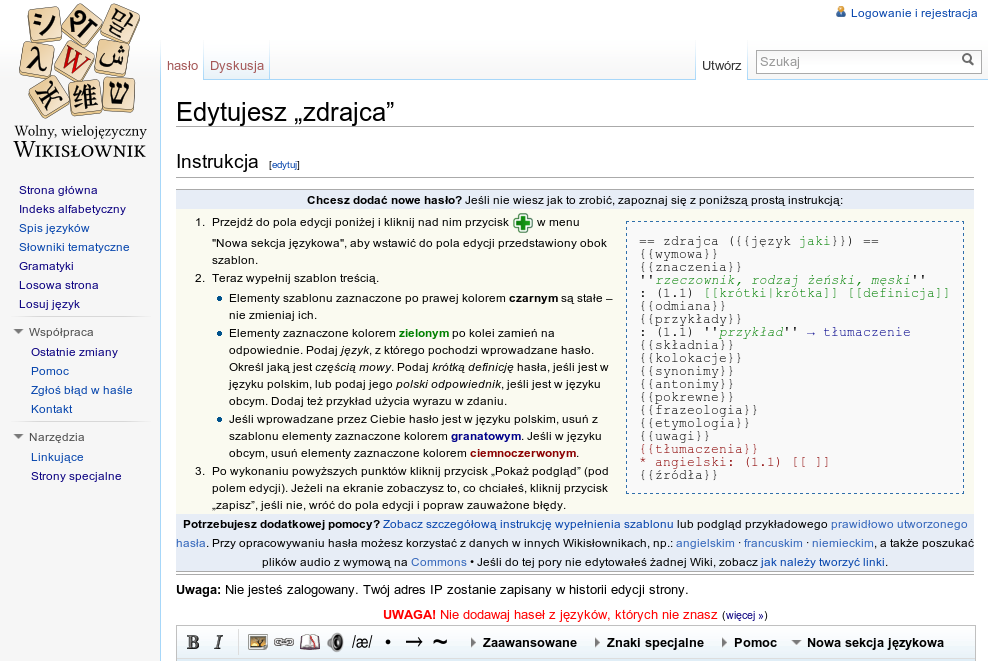
\includegraphics{plwikt-edit-non}}
	\caption{Próba stworzenia nowego hasła w~polskim Wikisłowniku}
	\label{fig:plnew}
\end{illustration}

Jak widać na zrzucie ekranu, sama instrukcja tworzenia nowego hasła jest na tyle skomplikowana, że może zniechęcić do edycji nowego redaktora. Wymagane jest skopiowanie podanego kodu i~pieczołowite podmienianie poszczególnych jego elementów. Niestety tylko w~bardzo ograniczonym stopniu uwzględniane jest, że niektóre języki mają zdecydowanie inną strukturę niż przykładowa. Osoba chcąca dodać do Wikisłownika nowy znak chiński będzie musiała nie tylko zapoznać się z~regułami dla tej specyficznej odmiany haseł, ale też prawdopodobnie skopiować kod istniejącego hasła z~tej kategorii. O~wiele lepsza byłaby sytuacja, w~której po wyborze języka edytujący otrzymuje odpowiedni szkielet hasła, który będzie mógł uzupełnić standardowym formularzem, bez potrzeby wybierania fragmentów, które należy zmienić lub usunąć.

Oparcie projektów Wikimedia na systemie MediaWiki i~wikikodzie powoduje tego typu problemy oczywiście nie tylko w~Wikisłowniku. Także w~Wikipedii komplikacje techniczne są dużą barierą dla nowych użytkowników, najczęściej przyzwyczajonych do narzędzi typu WYSIWYG (\emph{What You See Is What You Get}) takich jak Microsoft Word. W~badaniach przeprowadzonych w~2009~roku czytelnikom wszystkich wersji językowych Wikipedii zadano pytanie o~powody nieuczestniczenia w~pracach edycyjnych. 25,18\% spośród 21~492~ankietowanych odpowiedziało \emph{nie wiem, jak}, 12,49\% stwierdziło, że zbyt słabo zna używane technologie, natomiast 24,43\% wskazało, że obawiałoby się popełnienia błędu i~,,wpadnięcia w~kłopoty'' z~tego powodu (najczęściej wymienianym powodem było \emph{myślę, że nie mam wystarczającej wiedzy, którą mogę się podzielić} -- 51,98\%)~\cite{wiki:survey}. Wynika z~tego, że aż jedna czwarta czytelników, którzy wypełnili ankietę, to potencjalni redaktorzy, którzy nie angażują się w~tworzenie encyklopedii ze względu na uwarunkowania techniczne. Brak podobnych badań przeprowadzanych na użytkownikach Wikisłownika, można jednak przypuszczać, że kształtują się one podobnie. Dodatkowym czynnikiem jest specjalizacja projektu -- w~pracach przy słowniku w~dużej części uczestniczą lingwiści, którzy nie muszą biegle posługiwać się platformą MediaWiki.

W~przypadku Wikipedii od dawna podejmowane są wysiłki w~kierunku poprawienia obsługi technicznej serwisu. Istnieje np. alternatywny edytor haseł \emph{wikEd} dostępny dla każdego użytkownika po wybraniu w~preferencjach, w~ograniczonym zakresie wspomagający redagowanie haseł~\cite{wiki:wiked}. Prawdopodobnie jednak edytor WYSIWYG wspólny dla przedsięwzięć Fundacji Wikimedia nie powstanie w~przewidywalnej przyszłości. Z~tego powodu korzystne jest usprawnianie poszczególnych projektów z~uwzględnieniem ich cech charakterystycznych. Jednym z~celów opisanej aplikacji jest zwiększenie komfortu korzystania z~formularza wprowadzania haseł w~Wikisłowniku. Implementacja tego projektu została omówiona w~sekcji~\ref{sec:impl-form}.

Drugą znaczącą wadą Wikisłownika jest wynikająca z~wielojęzyczności ogromna redundancja, powodująca spore problemy dla czytelnika. Każda wersja językowa stanowi odrębną całość. Choć słowników internetowych nierzadko używają poligloci, którym może być obojętne, w~jakim języku zostaną zaprezentowane informacje, struktura Wikisłownika nie pozwala im wykorzystać swoich umiejętności. Specjalistyczne hasła mogą być dostępne np. wyłącznie w~jednej wersji językowej -- przeszukiwanie poszczególnych edycji to marnotrawienie czasu, dlatego często najlepszym rozwiązaniem bywa po prostu użycie wyszukiwarki, np. Google. Informacje w~różnych językach pojawiają się niezależnie od siebie, bowiem znakomita większość redaktorów jest aktywna wyłącznie w~jednym projekcie. Przy tym zdarza się, że wprowadzający informacje wykonuje zupełnie niepotrzebną pracę, którą ktoś wykonał wcześniej w~innej wersji językowej, a~nawet w~tej samej wersji, lecz podczas tworzenia innego hasła, w~pewien sposób powiązanego z~obecnie edytowanym.

Ważną funkcję we wszystkich projektach Wikimedia pełnią boty, odpowiadające w~największych projektach za od~10 do 30\% wszystkich edycji haseł ~\cite{bots}. W~polskim Wikisłowniku programy te przede wszystkim uzupełniają linki interwiki, ale także wykonują bardziej skomplikowane akcje: standaryzują układ podsekcji i~format linków, aktualizują indeksy i~inne listy słów oraz dodają polską wymowę~\cite{wikt:boty}~\cite{wikt:olafbot}. Część z~tych edycji jest wtórna i~spowodowana błędami popełnianymi przez początkujących redaktorów -- można by ich zatem uniknąć, usprawniając formularz edycji.

Automatyzacja edytora pozwala na sprawniejszą standaryzację i~użycie informacji wprowadzonych już do innych wersji językowych Wikisłownika. Bardzo pomocne okazuje się tu API MediaWiki~\cite{mw:api}. Ten interfejs programistyczny pozwala na sprawne pobieranie treści wybranych haseł z~dowolnego projektu Wikimedia w~celu dalszego przetwarzania. Zostało to wykorzystane podczas implementacji drugiej istotnej części aplikacji, a~następnie opisane w~sekcji~\ref{sec:impl-auto}.


\subsection{Różnice w~stosunku do Wikipedii}
Po analizie uwidacznia się odmienny charakter Wikisłownika w~stosunku do Wikipedii, która była pierwszym projektem Fundacji i~dziś jest jej sztandarowym przedsięwzięciem. W~tabeli~\ref{tab:wiki-wikt} zostały ujęte najważniejsze różnice między witrynami w~aspekcie technicznym.
\begin{table}[h]
\begin{center}
	\begin{tabularx}{\textwidth}{ XX }
		\toprule \textbf{Wikipedia} & \textbf{Wikisłownik} \\
		\toprule Struktura hasła różnorodna
			& Bardzo ściśle określona struktura hasła \\
		\midrule Przede wszystkim ciągły tekst
			& Listy, wypunktowania \\
		\midrule Umiarkowana liczba szablonów używanych w~hasłach w~stosunku do pozostałej treści
			& Bardzo duży udział szablonów w~treści hasła \\
		\midrule Duże różnice pomiędzy wersjami językowymi
			& Małe różnice pomiędzy wersjami językowymi \\
		\midrule Linki interwiki łączą informacje o~tym samym obiekcie w~różnych językach
			& Linki interwiki łączą informacje o~tym samym słowie występującym w~wielu językach, objaśnione w~różnych językach \\
		\midrule Nagłówki dzielą artykuł na sekcje o~dowolnej semantyce
			& Nagłówki dzielą artykuł na sekcje odpowiadające poszczególnym językom \\
		\bottomrule
	\end{tabularx}
\caption
	[Porównanie Wikipedii i~Wikisłownika -- aspekty techniczne]
	{Porównanie Wikipedii i~Wikisłownika -- aspekty techniczne. Zob. też tabelę \ref{tab:wiki-wikt2}}
\label{tab:wiki-wikt}
\end{center}
\end{table}

To wszystko powoduje, że usprawnienie edycji w~Wikisłowniku jest o~wiele łatwiejsze niż w~Wikipedii, której bardzo złożona struktura w~praktyce uniemożliwia dziś kompleksową przebudowę procesu redakcji. Ściśle określona struktura to ogromna zaleta projektu. Co ciekawe -- nie jest ona charakterystyczna dla wszystkich jego wersji językowych. Po części prac włożonych w~implementację okazało się, że polski Wikisłownik jest pod tym względem wyjątkowo dobrze zorganizowany. Wprawdzie wszystkie większe edycje zachowują standardowy podział na sekcje językowe, jednak owe sekcje niekiedy przybierają dość oryginalne postaci. Po dokładniejszej analizie można stwierdzić, że polski Wikisłownik jest wyjątkowo jednolity, co ma niebagatelne znaczenie zarówno dla czytelnika, jak i~dla edytora.


\chapter{Aspekty społecznościowe}
Tematem tego rozdziału są społecznościowe aspekty zarówno samego Wikisłownika, jak i~procesu powstawania niniejszej pracy magisterskiej. Na początku omówiono podstawowe założenia koncepcji \emph{wiki}, na której opiera się Wikisłownik. Kolejna część rozdziału to krótka analiza społeczności rozwijającej projekt. Na dalszych stronach znalazły się treści ściśle związane z~tworzoną aplikacją: opis rozwoju oprogramowania dla specyficznego klienta, jakim jest szersza społeczność, oraz szczegółowa analiza jego wymagań.

\section{Koncepcja \emph{wiki}}
Pojęcie \emph{wiki} określa witrynę internetową umożliwiającą tworzenie i~edycję dowolnej liczby połączonych ze sobą hiperłączami stron przez przeglądarkę internetową, za pomocą uproszczonego języka znaczników lub edytora WYSIWYG \cite{britannica}. Opisane w~rozdziale~\ref{chap:wikt} projekty Fundacji Wikimedia, szczególnie Wikipedia, są z~pewnością najbardziej znanymi i~największymi przykładami wiki.

Wiki to nie tylko technologia, ale także, a~może przede wszystkim, społeczność. Rozmiary wiki rozciągają się od małych, zamkniętych witryn firmowych do największej Wikipedii. To, co łączy wszystkie tego typu projekty, to otwarty dostęp do edycji i~tworzenia stron w~obrębie danej grupy. W~przypadku projektów Fundacji grupę tę stanowi niemal cała ludność świata dysponująca dostępem do internetu --- poza nielicznymi krajami, w~których sieć jest cenzurowana. Wśród redaktorów Wikipedii czy Wikisłownika nie istnieje żadna skodyfikowana hierarchia, co oznacza, że niezalogowany nowicjusz może zmienić stronę dokładnie tak samo jak administrator projektu. Założenie to od lat stanowi główny zarzut pod adresem Wikipedii --- negatywne opinie o~tej encyklopedii są szeroko rozpowszechnione i~chętnie cytowane przez jej przeciwników~\cite{knol}. Mimo tego projekty stale rozwijają się i~podnoszą swoją jakość --- już w~2005~roku w~czasopiśmie ,,Nature'' opublikowano kontrowersyjne porównanie Wikipedii z~\emph{Encyclopædia Britannica}, z~którego wynikało, że obie encyklopedie stoją na podobnym poziomie~\cite{nature:britannica}. Jasno widać, że znaczenie projektów Fundacji Wikimedia jest dziś bardzo duże.

W~tworzeniu Wikipedii i~Wikisłownika biorą udział przedstawiciele całego społeczeństwa --- w~pracach uczestniczą zarówno profesorowie, jak i~studenci. Jak wspomniano w~podrozdziale~\ref{wikt:drawbacks}, dla wielu z~nich barierą jest poziom skomplikowania oprogramowania MediaWiki. Podczas gdy wielu uczestników, najczęściej tych o~zainteresowaniach ścisłych, nie ma problemów z~opanowaniem techniki edycji haseł, istnieje duża grupa osób, które deklarują, że mogłyby zaangażować się bardziej, gdyby nie konieczność opanowania złożonych sposobów wprowadzania informacji. Dzięki regularnej strukturze akurat polski Wikisłownik jest tym projektem, w~którym uproszczenie tworzenia i~edycji haseł jest najbardziej możliwe do przeprowadzenia. Ponieważ proces taki wymaga wspólnej decyzji ogółu społeczności, należało zanalizować, jak kształtują się interakcje między użytkownikami w~projekcie.

\section{Społeczność polskiej edycji Wikisłownika}
\label{sec:plsoc}
W~punkcie~\ref{subs:wiki-wikt} przedstawione zostały różnice między technicznymi elementami polskich wersji Wikipedii i~Wikisłownika. Wysoki stopień uporządkowania haseł w~Wikisłowniku daje nadzieję na wprowadzenie ulepszeń --- główną potencjalną barierą może być więc społeczność, która stara się podejmować decyzje konsensualnie.

Dobrym sposobem przedstawienia społeczności Wikisłownika jest przeciwstawienie jej grupie osób edytujących w~Wikipedii\footnote{Od tej pory pojęcia \emph{Wikipedia} i~\emph{Wikisłownik} domyślnie oznaczać będą wersje polskojęzyczne.}. W~tabeli~\ref{tab:wiki-wikt2} przedstawiono najbardziej widoczne różnice między nimi, które można zauważyć już po kilkugodzinnej lekturze archiwalnych dyskusji i~historii edycji.

\begin{table}[h]
\begin{center}
	\begin{tabularx}{\textwidth}{ XX }
		\toprule \textbf{Wikipedia} & \textbf{Wikisłownik} \\
		\midrule Dużo wandalizmów (edycji wykonywanych w~złej wierze)
			& Bardzo mało wandalizmów \\
		\midrule Kilkuset stale aktywnych redaktorów
			& Kilkunastu stale aktywnych redaktorów \\
		\midrule Wielu użytkowników mających kłopoty z~dostosowaniem się do zasad
			& Niewielu użytkowników mających kłopoty z~dostosowaniem się do zasad \\
		\midrule Liczne wojny edycyjne (wzajemne cofanie swoich edycji przez co najmniej dwóch redaktorów)
			& Praktycznie brak wojen edycyjnych \\
		\midrule Niezliczone strony archiwalnych dyskusji
			& Łatwy dostęp do archiwalnych dyskusji \\
		\midrule Dobra dokumentacja i~pomoc
			& Dobra pomoc, ale szczegółowa dokumentacja bardzo uboga \\
		\midrule Bardzo zróżnicowane obszary zainteresowania
			& Społeczność o~wspólnych zainteresowaniach lingwistycznych \\
		\bottomrule
	\end{tabularx}
\caption
	[Porównanie Wikipedii i~Wikisłownika --- aspekty społecznościowe]
	{Porównanie Wikipedii i~Wikisłownika --- aspekty społecznościowe. Zob. też tabelę~\ref{tab:wiki-wikt}}
\label{tab:wiki-wikt2}
\end{center}
\end{table}
Można uznać, że w~przypadku polskich wersji językowych Wikisłownik jest projektem budzącym znacznie mniejsze emocje niż Wikipedia, której powszechność powoduje nieuniknione problemy, takie jak zaangażowanie osób chcących wykorzystać projekt do celów marketingowych lub ideologicznych czy liczne wandalizmy w~wykonaniu znudzonych nastolatków. Społeczność redaktorów słownika zdecydowanie skupiona jest na stałym udoskonalaniu projektu. Z~racji jego rozmiaru łatwiej jest o~konsensus w~dyskusjach, a~dzięki mniejszej popularności innowacyjne rozwiązania techniczne mają większą szansę na realizację.

W~polskim Wikisłowniku działa 26~administratorów, spośród których 14 jest aktywnych. Kilku z~nich obsługuje swoje własne boty~\cite{wikt:admin}. Dyskusje na ogólne tematy toczą się w~tzw. \emph{Barze} (odpowiedniku \emph{Kawiarenki} w~Wikipedii). Na podstawie strony specjalnej \emph{Ostatnie zmiany} można oszacować poziom aktywności redaktorów w~stosunku do Wikipedii. Podczas gdy tam ostatnie 500~zmian obejmuje nieco ponad godzinę, w~Wikisłowniku jest to więcej niż doba. Charakterystyczny jest dużo większy udział nowo tworzonych haseł w~stosunku do poprawek w~starszych artykułach niż w~Wikipedii. To dość naturalne --- hasła słownikowe są prostsze i~często nie wymagają dalszych poprawek technicznych po ich utworzeniu. Dużą część haseł tworzy mała, najbardziej aktywna liczba użytkowników: dłuższa obserwacja pozwala na stwierdzenie, że proporcje są mniej więcej zgodne z~zasadą Pareto (\emph{20\% obiektów jest związanych z~80\% zasobów}). Wynika z~tego, że warto stworzyć aplikację, która będzie służyć zarówno nowym użytkownikom (czego skutkiem będzie zwiększenie liczby zaangażowanych osób), jak i~tym doświadczonym, bardziej aktywnym (większa wydajność i~satysfakcja z~użytkowania).


\section{Analiza wymagań}
Aby sprecyzować elementy, które złożą się na implementację aplikacji, konieczne jest przeprowadzenie analizy wymagań. Ten proces pozwoli na zrozumienie dokładnych potrzeb, które powinny zostać spełnione, i~rozbicie ich na konkretne, jasno zdefiniowane wymagania~\cite{guidebook}. Klasyczne metody powinny być jednak nieco zmodyfikowane ze względu na specyfikę projektu --- odbiorcą nie jest klient biznesowy, ale społeczność skupiona wokół otwartego projektu (zob.~podrozdział~\ref{sec:spec}).

W~przypadku niniejszego projektu specyfikowanie wymagań prowadzone było w~ramach dyskusji w~\emph{Barze} na łamach Wikisłownika oraz prywatnych rozmów z~redaktorami. Dodatkowo swoje opinie przekazało kilka osób niezwiązanych z~projektem, mogących spojrzeć na zagadnienie z~punktu widzenia nowego użytkownika.

Najważniejszym produktem, będącym wynikiem analizy wymagań, jest specyfikacja wymagań biznesowych. Zgodnie z~klasycznym podziałem zostały one podzielone na wymagania funkcjonalne i~niefunkcjonalne.

\subsection{Definicje}

\begin{itemize}
\item \textbf{Użytkownik} --- osoba dokonująca edycji w~Wikisłowniku.
\item \textbf{Użytkownik zalogowany} --- osoba zalogowana w~Wikisłowniku i~dokonująca w~tym projekcie edycji.
\item \textbf{Użytkownik niezalogowany} --- osoba niezalogowana w~Wikisłowniku i~dokonująca w~tym projekcie edycji. Takie edycje zostaną zapisane wraz z~adresem IP użytkownika, co umożliwia częściową identyfikację autora.
\item \textbf{Przestrzeń nazw} --- grupa stron w~Wikisłowniku o~wspólnym prefiksie zakończonym dwukropkiem. Przykładowe przestrzenie nazw to \kod|Szablon:|, \kod|Dyskusja:|. Szczególnym przypadkiem jest tzw. przestrzeń główna, skupiająca strony bez dodatkowego prefiksu --- w~niej znajdują się wszystkie hasła słownika.
\item \textbf{Hasło} --- strona w~przestrzeni głównej Wikisłownika.
\item \textbf{Stary formularz} --- dotychczasowa metoda wprowadzania danych, opisana w~podrozdziale~\ref{wikt:structure}.
\item \textbf{Nowy formularz} --- aplikacja będąca przedmiotem niniejszej pracy.
\item \textbf{Sekcja} --- odcinek pojedynczego hasła dotyczący użycia słowa w~pojedynczym języku, wyróżniony nagłówkiem drugiego stopnia (\kod|==|).
\item \textbf{Podsekcja} --- element sekcji hasła zgodny z~ogólną strukturą haseł (p.~podrozdział~\ref{wikt:subsections}).
\item \textbf{Interwiki} --- linki pomiędzy poszczególnymi wersjami językowymi Wikisłownika.
\end{itemize}

\subsection{Wymagania funkcjonalne}
\subsubsection{Edycja istniejących haseł i~sekcji za pomocą nowego formularza}
Użytkownik musi mieć możliwość wprowadzenia zmian w~obrębie całego hasła Wikisłownika za pomocą nowego formularza. Formularz powinien umożliwiać edycję dowolnego elementu w~haśle --- w~szczególności dotyczy to sekcji wstępnej, zawierającej dane ogólne, niezwiązane z~żadnym językiem. Edycja ma polegać na uzupełnieniu wartości dla poszczególnych kluczy w~formularzu. Kluczami są tytuły kolejnych podsekcji, wartościami ich zawartość.

\subsubsection{Dodanie nowej sekcji do istniejącego hasła za pomocą nowego formularza}
Użytkownik musi mieć możliwość rozszerzenia istniejącego hasła o~kolejną sekcję językową. Sekcja powinna zostać automatycznie uzupełniona zawartością charakterystyczną dla wybranego języka.

\subsubsection{Utworzenie nowego hasła za pomocą nowego formularza}
Użytkownik musi mieć możliwość stworzenia nowego hasła, składającego się z~jednej lub wielu sekcji językowych. Każda sekcja powinna być utworzona w~sposób analogiczny do dodawania nowej sekcji do istniejącego hasła.

\subsubsection{Edycja i~utworzenie nowego hasła za pomocą starego formularza}
Użytkownik, który chce korzystać nadal ze starego formularza, musi mieć taką możliwość. Decyzja o~wyborze starego lub nowego formularza musi być łatwa do podjęcia i~możliwa do odwrócenia w~każdej chwili, także w~trakcie edycji lub tworzenia hasła.

\subsubsection{Wprowadzanie znaków specjalnych}
Użytkownik musi mieć możliwość prostego wprowadzania do formularza znaków specjalnych, w~szczególności liter alfabetów używanych w~językach opisywanych przez Wikisłownik.

\subsubsection{Usunięcie sekcji językowej}
Użytkownik musi mieć możliwość usunięcia dowolnej sekcji językowej z~hasła.

\subsubsection{Edycja tytułu sekcji językowej}
Użytkownik musi mieć możliwość zmiany tytułu sekcji językowej. Jest to konieczne z~powodu odrębnego traktowania haseł opisujących przysłowia, związki frazeologiczne i~inne wyrażenia składające się z~kilku wyrazów.

\subsubsection{Automatyczne pobieranie danych z~innych wersji językowych}
Użytkownik musi mieć możliwość wyszukania w~innych wersjach językowych Wikisłownika danych, które mogą być cennym uzupełnieniem edytowanego hasła. W~szczególności dotyczy to ilustracji, wymowy w~międzynarodowym alfabecie fonetycznym (IPA), nagrań dźwiękowych.%TODO UPDATE

\subsubsection{Automatyczne uzupełnianie podsekcji}
Aplikacja powinna automatycznie uzupełnić te spośród podsekcji w~danym haśle, które to umożliwiają. W~szczególności dotyczy to linków interwiki w~nowo dodawanej sekcji wstępnej, szablonów używanych do transliteracji, znacznika \kod|<references/>| w~podsekcji \emph{źródła}.%TODO UPDATE

\subsection{Wymagania niefunkcjonalne}
\subsubsection{Licencjonowanie}
Aplikacja musi zostać udostępniona na licencjach GNU~FDL~1.2 i~CC\dywiz{}BY\dywiz{}SA~3.0 --- wymagają tego zasady Wikisłownika i~wszystkich projektów Wikimedia. W~związku z~powyższym cały kod użyty w~aplikacji musi być dostępny już wcześniej na odpowiednich licencjach bądź udostępniony na nich przez autora pracy. Grafiki użyte w~interfejsie użytkownika muszą pochodzić z~serwisu Wikimedia Commons, zbierającego pliki na wolnych licencjach.

\subsubsection{Integracja z~Wikisłownikiem}
Aplikacja musi być w~pełni zintegrowana z~istniejącym interfejsem Wikisłownika. Z~tego powodu jedyną możliwą opcją jest aplikacja kliencka napisana w~języku JavaScript, w~rachubę nie wchodzi natomiast aplikacja desktopowa wymagająca dodatkowych czynności. Korzystanie z~nowego formularza powinno być inicjowane w~dokładnie ten sam sposób co korzystanie ze starego formularza.

\subsubsection{Pomoc kontekstowa}
Nowy formularz musi zawierać pomoc kontekstową dla wszystkich elementów, których działanie nie jest oczywiste. Wyświetlanie pomocy nie może utrudniać edycji hasła.

\subsubsection{Interfejs użytkownika}
Interfejs użytkownika musi być prosty, czytelny i~intuicyjny. W~szczególności bardzo istotne jest, aby dla nowego użytkownika nowy formularz stanowił duże ułatwienie i~zmniejszał barierę wejścia do projektu.

\subsubsection{Obsługiwane oprogramowanie}
Ponieważ Wikisłownik musi być dostępny do edycji dla jak największej liczby użytkowników, jest bardzo ważne, aby aplikacja obsługiwała wszystkie popularne przeglądarki internetowe: Firefox $\geq$~4, Chrome 13 (dzięki automatycznej aktualizacji w~przypadku tej przeglądarki nie występuje problem obsługi starszych wersji), Opera $\geq$~10 i~Internet Explorer $\geq$~7. W~przypadku braku wyłączonej obsługi JavaScriptu zachowanie formularza ma zostać niezmienione: załaduje się stary formularz z~wyłączonymi niektórymi funkcjami.

\subsubsection{Wydajność}
Aplikacja musi umożliwiać płynną pracę --- skrypty nie mogą być znacząco wolniejsze od skryptów użytych w~starym formularzu.

\subsubsection{Łatwość modyfikacji}
Ze względu na niestały charakter zasad panujących w~Wikisłowniku kod aplikacji musi być dostępny publicznie i~możliwy do modyfikacji w~każdej chwili. W~szczególności dotyczy to komunikatów dla użytkownika i~używanych stałych, które powinny być zebrane w~jednym miejscu.

\section{Specyfika tworzenia aplikacji dla wikispołeczności}
\label{sec:spec}
Opisywana aplikacja jest projektem dość szczególnym: nie powstaje na zamówienie klienta biznesowego, który mógłby określić dokładne wymagania. Ma także mało wspólnego z~klasycznymi projektami \emph{open source} --- z~założenia jej autorem jest jedna osoba, autor niniejszej pracy. Projekt formularza przyjmował coraz bardziej sprecyzowany kształt dzięki wypowiedziom członków otwartej społeczności i~ich wzajemnej dyskusji, duże znaczenie miały też testy wykonywane przez ochotników z~Wikisłownika. Aplikacja powstawała inkrementalnie, co kilka dni--tygodni skrypt na stronach Wikisłownika aktualizowany był do kolejnej działającej wersji z~nowymi funkcjami.

Dzięki takiemu modelowi budowy aplikacji na bieżąco wykrywane były błędy w~działaniu, o~które było łatwo ze względu na poziom skomplikowania kluczowych modułów takich jak parser wikitekstu. Projekt okazał się ciekawym doświadczeniem łączącym pozytywne cechy tworzenia oprogramowania dla klienta biznesowego i~programu na swój własny użytek.

Zarys projektu powstał jesienią 2010~roku w~wyniku pierwszej dyskusji w~\emph{Barze} Wikisłownika. Założona została wówczas podstrona poświęcona dyskusji wyłącznie temu zagadnieniu --- rozmowy w~ramach \emph{Baru} byłyby raczej niewygodne. Główny etap rozwoju aplikacji przypadł na okres od maja do września 2011~roku. W~toku dyskusji kilkukrotnie zmieniały się wymagania klienta, jakim jest wikispołeczność. W~tym wypadku, w~odróżnieniu od projektów biznesowych, cecha ta okazała się pozytywna. Dzięki bieżącym konsultacjom końcowy kształt aplikacji był satysfakcjonujący dla wszystkich stron uczestniczących w~przedsięwzięciu. Podrozdział~\ref{sec:impl-deploy} poświęcony jest ostatnim etapom projektu: wdrożeniu w~Wikisłowniku i~widokom na dalszy rozwój.


\chapter{Opis implementacji}
\label{chap:impl}
W~ostatnim rozdziale szczegółowo przedstawiony została implementacja aplikacji. Opisano użyte technologie i~metodologię, a~szczególną uwagę poświęcono problemom, które powstały podczas procesu tworzenia programu. Pierwsza sekcja zawiera opis środowiska, w~którym osadzona jest aplikacja, natomiast kolejne dwie skupiają się na dwóch logicznie wyodrębionych częściach projektu: uproszczonym formularzu edycyjnym oraz automatyzacji tworzenia haseł. W~ostatniej części rozdziału przedstawiono przebieg wdrożenia aplikacji w~polskim Wikisłowniku i~możliwości dalszego rozwoju.

Niniejszy rozdział zawiera odniesienia do plików źródłowych składających się na aplikację oraz pomocniczych. Wszystkie te pliki znajdują się na dołączonej do pracy płycie~CD w~katalogu \kod|src|.

\section{Wprowadzenie}
Oprogramowanie MediaWiki zostało napisane w~języku PHP (\emph{PHP Hypertext Preprocessor}) i~jest wysoce konfigurowalne za pomocą tzw. rozszerzeń, dodających kolejne funkcje --- przykładowo: obsługę przypisów, dodatkowe strony specjalne czy nowe funkcje parsera~\cite{mw:extensions}. W~projektach Fundacji obsługa rozszerzeń jest kontrolowana przez Fundację. Poszczególne projekty mogą składać prośby o~włączenie określonego rozszerzenia, decyzję podejmują zaś główni programiści Fundacji. Teoretycznie można rozważać utworzenie aplikacji dla Wikisłownika jako rozszerzenia w~PHP. Opcja ta została jednak odrzucona we wstępnej fazie projektu --- stworzenie rozszerzenia wymagałoby nieporównanie więcej formalności niż aplikacja kliencka, przede wszystkim jednak jego funkcjonalność byłaby znacznie ograniczona: poza polskim Wikisłownikiem żaden inny projekt nie mógłby z~niego skorzystać, na pewno nie zostałby więc włączony do głównej wersji MediaWiki.

\subsection{JavaScript w~Wikisłowniku}
Podobnie jak w~wielu innych przypadkach w~obrębie projektów Wikimedia jako metodę dostosowania silnika MediaWiki do szczególnych potrzeb wybrano zatem aplikację napisaną w~języku JavaScript (JS). Konieczne jest zatem przedstawienie sposobu obsługi skryptów na stronach tych witryn. Pliki JavaScript ładowane są z~wielu różnych źródeł --- hierarchia w~nieco uproszczonej postaci jest następująca~\cite{de:js}:
\begin{enumerate}
	\item skrypty systemowe oprogramowania MediaWiki, wspólne dla wszystkich projektów oraz charakterystyczne dla danego projektu ze względu na ładowane rozszerzenia,
	\item skrypt zapisany na poziomie danego projektu jako strona \kod|MediaWiki:Common.js| --- dostęp do niego mają lokalni administratorzy,
	\item skrypt zapisany na poziomie danego projektu dla wybranej przez użytkownika skórki (domyślną jest \emph{Vector}, poprzednią był \emph{Monobook}) jako strona, np. \kod|MediaWiki:Vector.js| --- dostęp do niego mają lokalni administratorzy,
	\item tzw. gadżety, czyli dodatkowe skrypty rozszerzające funkcjonalność, możliwe do włączenia w~preferencjach użytkownika --- także one edytowane i~wybierane są przez administratorów,
	\item skrypt zapisany na stronie danego użytkownika, np. \kod|User:Sokrates/common.js| --- na tym poziomie możliwe jest dostosowywanie skryptów do swoich potrzeb przez każdego użytkownika,
	\item skrypt zapisany na stronie danego użytkownika dla wybranej skórki, np. dla skórki \emph{Vector} --- \kod|User:Sokrates/vector.js|.
\end{enumerate}
Jak widać, możliwości dołączania dodatkowych skryptów są elastyczne i~dostępne na różnych poziomach dla różnych użytkowników. Decyzja o~włączeniu skryptów dla wszystkich użytkowników danego projektu należy do jego administratorów (nie licząc wspólnych skryptów narzuconych przez Fundację), natomiast każdy użytkownik poprzez edycję specjalnej strony może uruchamiać różne skrypty na swoje potrzeby, nie będąc zmuszonym do korzystania z~dodatków do przeglądarek, takich jak Greasemonkey. W~ten sposób ułatwiony jest proces powstawania i~testowania nowych skryptów: osoby chcące przetestować nowy skrypt mogą na swojej stronie JS dołączyć go do swojej. Jeśli administratorzy uznają skrypt za wartościowy, mogą go dodać do zbioru gadżetów (wtedy każdy użytkownik ma możliwość włączenia skryptu bez konieczności edycji plików JS) lub do ogólnego pliku \kod|MediaWiki:Common.js|.

\subsubsection{MediaWiki 1.17}
Projekty Fundacji od czerwca 2011~roku używają wersji MediaWiki~1.17. Wersja ta wprowadziła kilka istotnych zmian, spośród których najważniejszą było wprowadzenie modułu \kod|ResourceLoader|, zmieniającego system ładowania dodatkowych plików, przede wszystkim skryptów i~arkuszy stylów~\cite{mw:117}. Wszystkie potrzebne pliki są łączone w~jeden i~dodatkowo kompresowane, dodatkowo poprawiono też obsługę pamięci podręcznej po stronie klienta. Do tej pory poszczególne pliki JS i~CSS przesyłane były statycznie w~wielu żądaniach HTTP, co mogło powodować problemy z~ich synchronizacją, a~przede wszystkim zwiększało obciążenie sieci. Aktualizacja software'u projektów Fundacji spowodowała konieczność aktualizacji większości używanych w~nich skryptów i~zaangażowała większość aktywnych uczestników zaznajomionych z~technikaliami~\cite{mw:migration}.

Od wersji~1.16 do MediaWiki dołączana jest biblioteka programistyczna jQuery, a~w~najnowszym wydaniu zaktualizowano ją do wersji 1.4.2~\cite{mw:jquery}. Jest to jedna z~najczęściej używanych bibliotek dla JavaScriptu, w~bardzo dużym stopniu usprawniająca programowanie w~tym języku. Kod pisany za jej pomocą jest o~wiele czytelniejszy i~prostszy, biblioteka pozwala też wyeliminować wiele problemów związanych z~nieprawidłową obsługą JavaScript w~niektórych przeglądarkach~\cite{jquery:action}~\cite{jquery:doc}.

\subsection{Środowisko programistyczne}
Programowanie w~języku JavaScript wymaga użycia innych metod niż tworzenie aplikacji desktopowych. Do tworzenia edytora dla Wikisłownika użyto m.in. następujących aplikacji:

\subsubsection{Geany}
Lekkie zintegrowane środowisko programistyczne (IDE)~\cite{geany}. W~początkowej fazie projektu używane było środowisko Eclipse z~dodatkowymi wtyczkami --- okazało się jednak, że obsługa JavaScriptu nie jest w~nim na tyle wygodna, aby konieczne było wykorzystywanie tak rozbudowanego edytora.
\subsubsection{Przeglądarki internetowe}
Aplikacja została przetestowana w~przeglądarkach Firefox $\geq$~4, Chrome 13, Opera $\geq$~10 i~Internet Explorer $\geq$~7, pod systemami operacyjnymi Linux i~Windows. Wyeliminowano błędy, które zostały odkryte w~czasie testów. W~trakcie implementacji używane były przeglądarki Google Chrome (i~jej wbudowane narzędzia deweloperskie) oraz Firefox z~dodatkiem Firebug, ułatwiającym debugowanie aplikacji~\cite{firebug}. Prawidłowe działanie aplikacji pod maksymalną możliwą liczbą dostępnych przeglądarek jest kluczowe ze względu na jej charakter --- edycja jest dostępna dla każdego użytkownika. Nie testowano jednak edytora w~starszych wersjach tych programów ze względu na ich znikome rozpowszechnienie i~niewspółmierny koszt takich testów w~stosunku do spodziewanych korzyści.
\subsubsection{Git}
Systemem kontroli wersji używanym w~projekcie był Git. Dzięki niemu możliwe było uniknięcie jakichkolwiek problemów związanych z~zarządzaniem wersjami. Dla bezpieczeństwa kod był na bieżąco wysyłany do zdalnego repozytorium założonym w~serwisie GitHub~\cite{github}. Kontroli wersji podlegała również niniejsza praca i~jej kod źródłowy w~systemie \XeTeX. Historia zmian aplikacji i~pracy jest dostępna do wglądu na serwerach GitHub~\cite{github:wikt}.
\subsubsection{The Regex Coach}
W~aplikacji duże znaczenie odgrywają wyrażenia regularne, wykorzystywane podczas parsowania wikitekstu. The Regex Coach jest programem ułatwiającym konstruowanie poprawnych wyrażeń~\cite{regexcoach}.
\spacer

\subsection{Dobre praktyki}
Nowy edytor został napisany za pomocą biblioteki jQuery, co ułatwia utrzymanie dobrej struktury. Kod podzielono na moduły funkcjonalne, co częściowo stanowi odpowiednik klasycznego paradygmatu obiektowego, często stosowany w~przypadku JavaScriptu. Język ten umożliwia pisanie aplikacji przy zachowaniu wielu różnych paradygmatów. W~przypadku opisywanej aplikacji zdecydowano się na wspomniany podział na moduły, będący pewnym kompromisem między paradygmatem funkcyjnym i~obiektowym. Moduły zaimplementowane są jako obiekty, których elementami są funkcje odpowiedzialne za operacje działające w~podobnym zakresie. Przykładowo parser wikitekstu jest modułem o~następującej strukturze:

\begin{jscode}{code:module}{Ogólna struktura modułu JavaScript}
var EParser = {
	getSections : function (code) {
		...
	},
	getSectionFromTitle : function (str) {
		...
	},
	getTitleFromCode : function (code) {
		...
	},
	...
};
\end{jscode}
Podział na moduły ułatwia uwzględnienie niektórych spośród licznych praktyk zalecanych przy programowaniu w~języku JavaScript. Istnieje kilka narzędzi, które w~automatyczny sposób badają jakość kodu skryptów, pomagając znaleźć potencjalne błędy i~uniknąć kolejnych. Podczas implementacji stale korzystano z~trzech z~nich: JSHint~\cite{jshint:doc}, JavaScriptLint~\cite{javascriptlint:doc}, a~przede wszystkim JSLint~\cite{jslint:doc}. Narzędzia te nie są do końca kompatybilne ze sobą nawzajem, dlatego za cel obrano całkowity brak ostrzeżeń generowanych przez JSLint. W~ten sposób udało się utrzymać m.in. następujące elementy:
\begin{itemize}
	\item kontrola nad zmiennymi globalnymi (w~przeciwieństwie do innych języków, np. PHP, domyślna deklaracja zmiennej bez słowa kluczowego \kod|var| powoduje umieszczenie jej w~zakresie globalnym),
	\item kończenie poleceń średnikiem (ich brak może prowadzić do błędów bardzo trudnych do wykrycia),
	\item odpowiednie tworzenie bloków kodu,
	\item sprawdzanie \kod|if (object.hasOwnProperty(name))| wewnątrz pętli \kod|for name in object| (z~powodu rozszerzalności prototypów funkcji brak takiego obostrzenia prowadzi do błędów),
	\item prawidłowe używanie operatorów takich jak \kod|===|, \kod|!==|,
	\item prawidłowe używanie konstruktorów,
	\item spójne wcięcia i~używanie nawiasów.
\end{itemize}

Istotnym zagadnieniem jest podział kodu na pliki. Podczas gdy w~trakcie implementacji oczywiste jest, że podział na moduły powinien implikować także podział na pliki, na cele testowania aplikacji przez społeczność o~wiele wygodniejsze jest używanie jednego pliku zawierającego jej całość --- w~przeciwnym razie konieczne byłoby stałe edytowanie większej liczby stron specjalnych Wikisłownika. Używanie wielu plików powoduje też problemy z~synchronizacją ich ładowania, ponieważ funkcja inicjalizująca aplikację powinna zostać uruchomiona dopiero po wczytaniu całości aplikacji.

Po rozważeniu kilku możliwości zdecydowano się na użycie skryptu \kod|make.sh| napisanego w~Bashu, łączącego wszystkie pliki aplikacji w~jeden, który okresowo był aktualizowany na stronie \url{http://pl.wiktionary.org/wiki/Wikipedysta:ToSter/ed.onefile.js}. Dodatkowym problemem było dołączenie kodu CSS: standardową metodą używaną w~Wikisłowniku byłoby utworzenie oddzielnej strony zakończonej na \kod|.css| i~ładowanie jej razem ze stroną \kod|.js|. W~skrypcie budującym wynikowy kod użyto jednak innej techniki --- arkusz stylów z~lokalnego pliku \kod|.css| był przetwarzany w~sposób umożliwiający dynamiczne dodanie go do zawartości strony jako łańcuch znaków. Skrypt \kod|make.sh| wykonywał też kilka innych czynności: opatrywał program adnotacjami dla JSLint, usuwał zbędne spacje i~znaczniki BOM w~plikach Unicode oraz zamykał całość aplikacji w~domknięciu JavaScript (\emph{closure}).

Kod aplikacji jest w~maksymalnie możliwym zakresie zgodny z~konwencjami przyjętymi przez programistów MediaWiki na potrzeby wewnętrznych części systemu~\cite{mw:conventions}.

\section{Formularz edycyjny}
\label{sec:impl-form}

Jedną z~dwóch głównych części aplikacji jest nowy formularz, usprawniający w~znacznym zakresie proces edycji i~tworzenia nowych artykułów. Do tej pory cały ów proces polegał na wpisywaniu, kopiowaniu i~uzupełnianiu wikikodu (por.~ilustracja~\ref{fig:plhaslo-edit}), a~najprostszym rozwiązaniem często okazywało się kopiowanie go z~innego, podobnego hasła i~modyfikowanie jedynie zmieniających się elementów. Dlatego też większość haseł w~Wikisłowniku powstawała seriami --- tworzenie pojedynczych haseł było niepraktyczne, natomiast wstawianie podobnego kodu do dziesiątek haseł dość łatwe do przeprowadzenia. Jako że każda sekcja językowa hasła składa się w~rzeczywistości z~par klucz--wartość, wygodniejszym sposobem wprowadzania danych byłby klasyczny formularz, do wypełniania jakiego przyzwyczajony jest każdy internauta. Nowy edytor został zatem zaprojektowany właśnie w~taki sposób, dzięki czemu zmniejsza się bariera wejścia dla początkującego redaktora. Od tej pory edycja hasła będzie polegać nie na wpisywaniu dość skomplikowanego kodu, co jest porównywalne z~prostym programowaniem, ale na wypełnieniu formularza.

Implementacja formularza składa się z~kilku modułów, spośród których główną rolę odgrywają \kod|EUi| w~pliku \kod|ed.ui.js| (interfejs użytkownika), \kod|EParser| i~\kod|ESectionParser| w~pliku \kod|ed.parser.js| (parser wikitekstu) oraz \kod|EPrinter| w~pliku \kod|ed.printer.js| (drukowanie danych przetworzonych przez aplikację). Poniżej opisano te moduły, szczególnie uwzględniając powstałe problemy i~ich rozwiązania.

\subsection{Interfejs użytkownika}
Kluczowym elementem projektu i~implementacji aplikacji jest interfejs użytkownika --- to jego jakość stanowi o~końcowym powodzeniu przedsięwzięcia. Szczególnie ważna jest bezproblemowa integracja nowego formularza z~dotychczasowym interfejsem. Wszystkie dotychczasowe funkcje używane w~trybie edycji, których zastosowanie miałoby sens i~w~nowej wersji, muszą pozostać dostępne.

%Zrzuty ekranu nowego formularza załączono w~dodatku~\ref{app:screen}.

\begin{illustration}
	\fbox{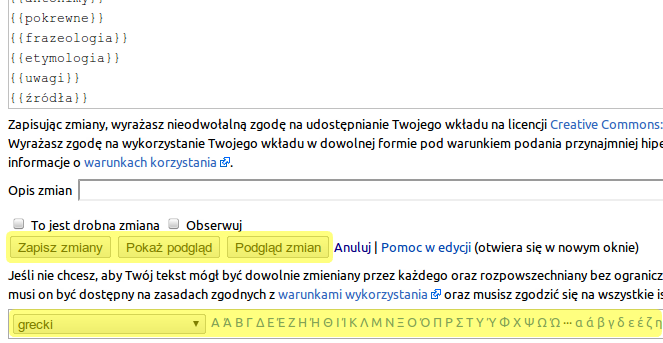
\includegraphics{edit-bottom-desc}}
	\caption{Kluczowe elementy interfejsu w~trybie edycji}
	\label{fig:edit-bottom}
\end{illustration}

Podstawowym problemem, powstałym na początku implementacji, było podpięcie nowego formularza pod mechanizmy przetwarzające dane po stronie serwera. Z~powodu braku jakiegokolwiek dostępu do konfiguracji serwera konieczne jest zapewnienie prawidłowego jego działania jedynie przy użyciu JavaScriptu. Na ilustracji~\ref{fig:edit-bottom} wyróżniono m.in. najważniejsze elementy sterujące edycją hasła. Są to trzy przyciski, których wybór powoduje wysłanie formularza w~trybie \kod|POST| na serwer do strony \kod|index.php| --- dalsze akcje uzależnione są od tego, który przycisk wybrano. Nową treścią hasła staje się zawartość głównego pola typu \kod|<textarea>|, o~identyfikatorze \kod|name="wpTextbox1"|. W~celu zapewnienia działania nowego formularza zgodnie z~oprogramowaniem MediaWiki możliwe były dwie opcje:
\begin{enumerate}
\item Usunięcie standardowych elementów, przede wszystkim pola \kod|wpTextbox1|, i~zastąpienie ich własnymi. Konieczne byłoby stworzenie pola formularza o~nazwie \kod|wpTextbox1| --- mogłoby to być pole ukryte (\kod|<input type="hidden" />|), które musiałoby być synchronizowane z~polami nowego formularza.
\item Ukrycie standardowych elementów i~synchronizacja zawartości pola \kod|wpTextbox1| z~polami nowego formularza.
\end{enumerate}
Wybór padł na rozwiązanie drugie z~kilku powodów. Okazało się, że dostęp do standardowych elementów w~trakcie działania nowego formularza jest bardzo przydatny, przede wszystkim zaś ich ukrywanie (za pomocą metody jQuery \kod|.hide()|, zmieniającej atrybut CSS \kod|display| na \kod|none|) umożliwia proste przełączanie między starym a~nowym formularzem w~trakcie edycji, co było jednym z~wymagań funkcjonalnych aplikacji. Należało zatem zapewnić prawidłową synchronizację pomiędzy polem \kod|wpTextbox1| a~polami nowego formularza. Najważniejsze było podpięcie odpowiednich zdarzeń pod przyciski wysyłające formularz na serwer, co widoczne jest na listingu~\ref{code:rebind}.

\begin{jscode}{code:rebind}{Funkcja \kod|EUi.rebindFormActions|}
rebindFormActions : function () {
    this.form.find('textarea').removeAttr('name');
    $('form').submit(function () {
	    if (EUi.usingNew) {
			EUi.deleteEmptySections();
			EUi.tbox.val(EPrinter.recalculateCode());
		}
		return true;
	});
}
\end{jscode}%$

W~momencie próby wysłania formularza na serwer skrypt sprawdza, czy użyty jest nowy formularz. W~takim przypadku ukryte okno tekstowe starego formularza, zapisane jako zmienna \kod|EUi.tbox|, wypełniane jest nową zawartością. Za jej obliczenie odpowiada funkcja \kod|EPrinter.recalculateCode|, opisana w~podsekcji~\ref{impl:parser}. Dzięki usunięciu atrybutów \kod|name| ze wszystkich pól tekstowych w~obrębie nowego formularza redukowana jest ilość przesyłanych danych, a~z~punktu widzenia serwera nic się nie zmienia.

Z~kolei po zmianach wprowadzonych za pomocą starego formularza konieczne jest ponowne parsowanie wikikodu, które jest wykonywane w~identyczny sposób jak przy inicjowaniu nowego edytora.

\begin{illustration}
	\fbox{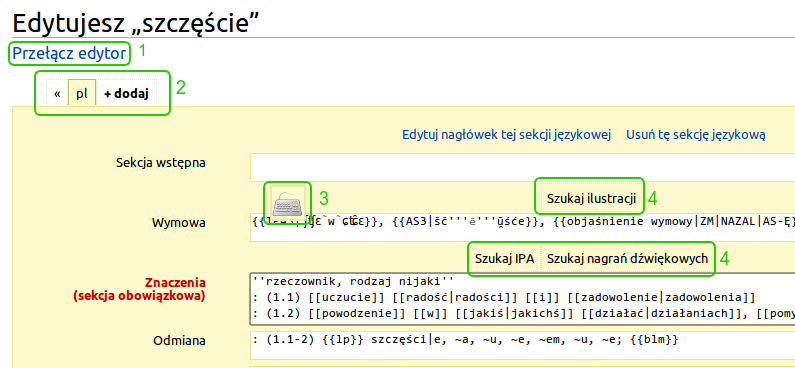
\includegraphics{newform-desc}}
	\caption{Fragment nowego formularza w~haśle z~jedną sekcją językową}
	\label{fig:newform}
\end{illustration}

Zrzut ekranu~\ref{fig:newform} przedstawia podstawowe elementy interfejsu nowego formularza:
\begin{enumerate}
\item Link pozwalający na przełączanie pomiędzy nowym a~starym edytorem,
\item Zakładki odpowiadające poszczególnym sekcjom językowym. Za podział na sekcje odpowiada moduł \kod|EParser|, natomiast zadaniem modułu \kod|EUi| jest ich odpowiednie wyświetlenie. Każdej sekcji odpowiada element \kod|<fieldset>| zawierający pola tekstowe z~poszczególnymi podsekcjami. Górne zakładki pozwalają na przełączanie pomiędzy sekcjami --- w~ten sposób redaktor widzi tylko tę sekcję, którą chce w~danym momencie edytować. W~starym formularzu konieczne było odnalezienie odpowiedniego kawałka kodu.

Sekcje językowe oznaczone są kodami ISO stosowanymi powszechnie w~Wikisłowniku. Oczywiście nie wszystkie kody są intuicyjne, dlatego po najechaniu myszą na każdą zakładkę pojawia się dokładna podpowiedź na temat danej sekcji.

Do zakładek językowych dodane są także zakładki o~specjalnej funkcji: pierwsza z~nich pozwala na edycję sekcji wstępnej (zawierającej m.in. interwiki), druga umożliwia dodanie nowej sekcji (pojawia się wówczas okno dialogowe z~zapytaniem o~język nowej sekcji).
\item Podręczna klawiaturka umożliwiająca wprowadzanie dużą liczbę znaków specjalnych do obecnie edytowanego pola. Podobna klawiaturka znajduje się w~starym edytorze --- została oznaczona kolorem żółtym na ilustracji~\ref{fig:edit-bottom}. W~nowym formularzu funkcja ta została usprawniona. Udało się wykorzystać istniejące już skrypty i~zintegrować z~aplikacją. Listing~\ref{code:specialchars} przedstawia moduł \kod|ESpecialChars|, odpowiadający za przemieszczanie elementów HTML pomiędzy nowym a~starym formularzem.
\item Przyciski pod poszczególnymi polami formularza pozwalają na automatyzację pewnych akcji. Ich działanie opisano w~sekcji~\ref{sec:impl-auto}.
\end{enumerate}

\begin{jscode}{code:specialchars}{Moduł \kod|ESpecialChars|}
ESpecialChars = {
	/* element HTML zawierajacy klawiaturke */
	obj : undefined,
	/* dotychczasowy element-rodzic klawiaturki */
	formerParent : undefined,
	detached : 0,

	/* odlaczenie klawiaturki od starego edytora i dodanie do elementu keyboard_keys w nowym formularzu */
	detach : function () {
		var container;
		if (ESpecialChars.detached) {
			return;
		}
		container = $('#keyboard_keys');
		ESpecialChars.obj = $('#editpage-specialchars');
		ESpecialChars.formerParent = ESpecialChars.obj.parent();
		ESpecialChars.obj.detach();

		container.append(ESpecialChars.obj);
		ESpecialChars.detached = 1;
	},

	/* ponowne przylaczenie klawiaturki do starego rodzica */
	attach : function () {
		if (!ESpecialChars.detached) {
			return;
		}
		EKeyboard.hide();
		ESpecialChars.obj.detach();
		ESpecialChars.formerParent.append(ESpecialChars.obj);
		ESpecialChars.detached = 0;
	},

	toggle : function () {
		if (ESpecialChars.detached) {
			ESpecialChars.attach();
		} else {
			ESpecialChars.detach();
		}
	}
};
\end{jscode}

Na ilustracji~\ref{fig:keyboard} pokazano działanie klawiaturki ekranowej w~nowym formularzu. Klawiaturę włącza się i~wyłącza kliknięciem w~ikonę z~klawiaturą, widoczną pod aktywnym właśnie polem tekstowym. Oprócz zawartości dostępnej w~starym formularzu można też wybrać jeden z~najczęściej używanych znaków. Ta funkcja znacząco usprawniła proces tworzenia haseł w~językach używających innych alfabetów lub znaków diakrytycznych. Stan klawiatury ekranowej (włączona/wyłączona) zapamiętywany jest w~ciasteczku przeglądarki, zostaje więc zachowany na kolejnych stronach.

\begin{illustration}
	\fbox{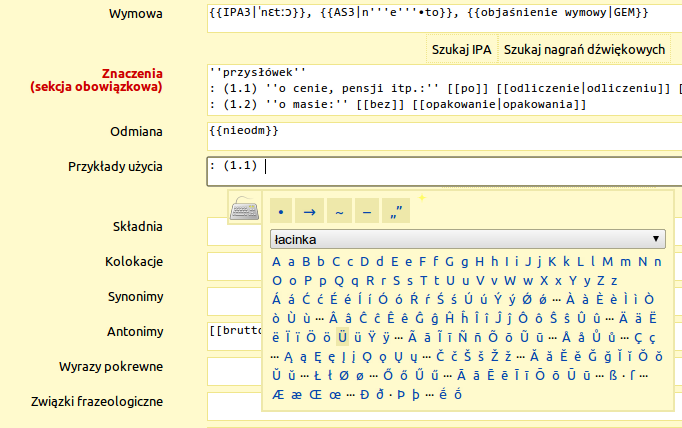
\includegraphics{edit-keyboard}}
	\caption{Użycie klawiaturki ekranowej w~nowym formularzu}
	\label{fig:keyboard}
\end{illustration}

Ciekawym problemem było ułożenie pól formularza w~taki sposób, by zajmował możliwie mało miejsca, a przy tym pozostał przejrzysty. Każda sekcja językowa składa się z~kilkunastu podsekcji, dlatego należało dobrze rozmieścić kilkanaście pól tekstowych, przy czym te mogły zawierać bardzo dużo tekstu (np. podsekcja \emph{tłumaczenia} w~popularnych polskich hasłach) albo i~pozostawać puste. Najprostszym, standardowym rozwiązaniem byłoby ustawienie stałej wysokości (np. równej 3~wierszom) dla każdego pola, które byłoby wyposażone w~zwykły pasek przewijania. Takie pola w~większości przypadków zajmowałyby jednak o~wiele za dużo miejsca, przy tym formularz z~dużymi białymi plamami jest niezbyt estetyczny. Zdecydowano się na rozwiązanie spotykane czasem w~portalach internetowych, najlepiej znane z~Facebooka --- pola tekstowe zmieniają swój rozmiar w~trakcie wpisywania kolejnych znaków. Istnieje kilka wtyczek do jQuery o~podobnej funkcjonalności, jednak na potrzeby aplikacji konieczne było stworzenie takiej, która łączy cechy kilku z~nich. Problemem okazała się też wydajność, ponieważ niektóre hasła mają w~trybie edycji nawet ponad sto pól dynamicznie dostosowujących swój rozmiar. Rozwiązaniem jest dołączenie do strony ukrytego elementu \kod|<div>|, do którego na bieżąco kopiowana jest zawartość ukrytego pola tekstowego --- na podstawie jego wysokości ustawiana jest wysokość pola. Kod przedstawiony jest na listingu~\ref{code:autoresize}.

\begin{jscode}{code:autoresize}{Wtyczka jQuery odpowiadająca za zmianę rozmiaru pól tekstowych}
/* wzorowane na https://github.com/jaz303/jquery-grab-bag/raw/master/javascripts/jquery.autogrow-textarea.js */
(function ($) {
	$.fn.autoresize = function () {
		var shadow = $('<div/>').css({
				position: 'absolute',
				top: -10000,
				left: -10000,
				resize: 'none'
			}).appendTo(document.body);

		this.filter('textarea').each(function () {
			var $this = $(this), minHeight = 25, maxHeight = 500,
				prevHeight = 0, nowHeight = 0;
			var update = function () {
				var val = this.value.replace(/[<>&]/g, 'w').replace(/\n$/, '<br/>&nbsp;').replace(/\n/g, '<br/>');
				shadow.html(val);
				nowHeight = Math.min(Math.max(shadow.height(), minHeight), maxHeight);
				if (nowHeight !== prevHeight) {
					$(this).css('height', nowHeight);
					EKeyboard.updatePosition($(this));
					prevHeight = nowHeight;
				}
			};

			shadow.css({
				width: $(this).width() - parseInt($this.css('paddingLeft'), 10) - parseInt($this.css('paddingRight'), 10),
				fontSize: $this.css('fontSize'),
				fontFamily: $this.css('fontFamily'),
				lineHeight: $this.css('lineHeight')
			});
			$(this).keyup(update).blur(update).focus(update);
			update.apply(this);
		});
		return this;
	};
}(jQuery));
\end{jscode}%$

Innymi usprawnieniami interfejsu użytkownika w~aplikacji są np.:
\begin{itemize}
\item Podpowiedzi pojawiające się po najechaniu myszką na część elementów strony. Aby ułatwić ich tworzenie, powstała wtyczka do jQuery. Dzięki jej użyciu aby dodać podpowiedź do dowolnego elementu HTML, wystarczyło nadać jej klasę CSS \kod|tip| i~treść podpowiedzi nadać za pomocą metody jQuery \kod|.data('tip', 'Odpowiedni tekst')|.
\item Okna dialogowe zastępujące standardowe funkcje typu \kod|alert|, \kod|confirm|, \kod|prompt|. Pojawiające się w~obrębie strony okno można dowolnie modyfikować.
\end{itemize}

\subsection{Parsowanie i~drukowanie wikitekstu}
\label{impl:parser}
Fundamentalne znaczenie dla aplikacji ma moduł odpowiadający za parsowanie wikitekstu --- kodu źródłowego haseł. O~trudności zagadnienia niech świadczy fakt, że przez ponad 10~lat istnienia Wikipedii nie udało się stworzyć edytora WYSIWYG --- i~prawdopodobnie w~dalszym ciągu nie będzie to wykonalne ze względu na coraz większy poziom skomplikowania artykułów. Tylko dzięki wyjątkowo przejrzystej strukturze polskiego Wikisłownika udało się stworzyć aplikację. Warto zaznaczyć, że kilka lat temu także polska edycja internetowego słownika nie nadawała się do tego typu projektu --- hasła udało się uprzątnąć za pomocą botów sterowanych przez kilka osób, które włożyły w~to dużo wysiłku.

Najistotniejszą funkcją parsera jest podział hasła na sekcje językowe, a~następnie na podsekcje --- zgodnie z~ogólnym schematem danego języka. Dzięki dobrej obsłudze wyrażeń regularnych w~JS kod odpowiadający za to jest dość krótki, jednak stworzenie prawidłowo działającej aplikacji wymagało długich testów, przeprowadzanych zarówno przez autora, jak i~społeczność Wikisłownika.

O~ile parsowanie hasła odbywa się według jasnych reguł, o~tyle generowanie wikitekstu z~poszczególnych fragmentów artykułu okazało się o~wiele trudniejsze. Problemem nie było stworzenie kodu, który byłby poprawny, ale zadbanie o~to, by aplikacja nie powodowała zbędnych zmian w~kodzie. Kluczowa jest funkcja \kod|EPrinter.recalculateCode|, zaprezentowana w~wersji uproszczonej na listingu~\ref{code:recalculate}.

\begin{jscode}{code:recalculate}{Funkcja \kod|EPrinter.recalculateCode|}
recalculateCode : function () {
	var id, sec, i, j, subs,
		code = [],
		sortableSections = [];
	...
	/* sortableSections zawiera spis tych sekcji, ktore maja znalezc sie w hasle */
	/* kolejne kawalki kodu dodawane sa do tablicy code, ktora na koniec jest laczona w jeden lancuch znakow */
	for (i in sortableSections) {
		if (sortableSections.hasOwnProperty(i)) {
			sec = sortableSections[i];
			if (sec.id === EConstants.SECTION_ID_INTRO) {
				/* sekcja wstepna */
				/* EUi.val() pobiera zawartosc pola tekstowego w formularzu */
				code.push(EUi.val(EConstants.SECTION_ID_INTRO, '') + '\n');
			} else {
				/* tytul sekcji */
				code.push('== ' + sec.title + ' ==\n');
				/* poszczegolne podsekcje */
				for (j = 0; j < sec.subsections.length; j += 1) {
					subs = sec.subsections[j];
					if (subs.active) {
						subs.content = EUi.val(sec.id, subs.title);

						if (!subs.title && subs.content) {
							/* podsekcja wstepna */
							code.push(subs.content + '\n');
						} else if (subs.title && !subs.content) {
							/* pusta podsekcja */
							code.push('{{' + subs.title + '}}\n');
						} else ... {
							code.push('{{' + subs.title + '}}' + EPrinter.adequateWhitespace(subs) + subs.content + '\n');
						}
					}
				}
				code.push('\n');
			}
		}
	}
	/* laczenie w jeden napis i usuniecie wielokrotnych spacji */
	return $.trim(code.join('')).replace(/ {2,}/g, ' ');
}
\end{jscode}%$

Ciekawa jest funkcja \kod|EPrinter.adequateWhitespace|, użyta w~powyższym kodzie w~części odpowiadającej za wydrukowanie danej podsekcji. Jak się okazało, sposób drukowania poszczególnych podsekcji nie jest jednorodny. Za każdym razem istnieje kilka możliwości:
\begin{itemize}
\item Zawartość podsekcji zaczyna się od nowej linii.
\item Zawartość podsekcji zaczyna się od spacji.
\item Zawartość podsekcji zaczyna się od nowej linii i~dwukropka ze spacją (\kod|: |) powodującego wcięcie tekstu.
\end{itemize}

Aby ustalić, który wzorzec wybrać, trzeba wziąć pod uwagę wiele warunków. Na listingu~\ref{code:whitespace} przedstawiono funkcję to realizującą, opatrzoną dokładnymi komentarzami.

\begin{jscode}{code:whitespace}{Funkcja \kod|EPrinter.adequateWhitespace|}
adequateWhitespace : function (subsection) {
	var str = subsection.content;
	/*
	 * Teksty zaczynajace sie od dwukropka, gwiazdki, zaczynajace sie od "<references", "{{litera|", "{{kolor|", szablony zaczynajace sie na "{{zch-", linki do grafiki (file:, grafika: image: media: plik:, to samo duza litera, mozliwe biale znaki miedzy nawiasami kwadratowymi a tym slowem),...
	 */
	if (str.search(/[:\*#]|<references|\{\{(litera|kolor)\||\{\{zch-|\[\[(file|image|grafika|plik|media):/i) === 0) {
		return '\n';
	}
	/*
	 * ...teksty w polach "znaczenia", "przyklady" oraz "tlumaczenia" nie moga wystepowac zaraz po szablonie, jesli wystepuja, musza byc przeniesione bez dodawania dwukropka.
	 */
	if (EConstants.SUBSECTIONS_WITH_NL.indexOf(subsection.title) !== -1) {
		return '\n';
	}
	/*
	 * Inne teksty skladajace sie z wiecej niz jednej linii powinny byc przeniesione z dodaniem dwukropka i spacji na poczatku pierwszej linii
	 */
	if (str.indexOf('\n') !== -1 && str.search(/[:\*#]/) !== 0) {
		return '\n: ';
	}
	/*
	 * Wpp: dla wypelnionych przed edycja pol zachowujemy istniejace formatowanie, o ile dane pole juz bylo niepuste.
	*/
	if (subsection.initcontent) {
		return subsection.initmultiline ? '\n: ' : ' ';
	}
	/*
	 * w polach pustych przed edycja: w sekcjach "wymowa", "transliteracja", "transkrypcja", "ortografie", "klucz", "kreski", "czytania", "hanja-kreski" defaultem jest pisanie bezposrednio po szablonie (po spacji)...
	 */
	if (EConstants.SUBSECTIONS_WITHOUT_NL.indexOf(subsection.title) !== -1) {
		return ' ';
	}
	/*
	 * a w pozostalych od nastepnej linii (jesli nie jest to "znaczenie" ani pierwsza sekcja ani "przyklady", ani "tlumaczenia", a tekst nie zaczyna sie od dwukropka lub gwiazdki, to program powinien sam dodac dwukropek i spacje)
	 */
	return '\n: ';
}
\end{jscode}

Moduł \kod|EPrinter| odpowiada także za generowanie kodu z~danych pobranych w~sposób automatyczny. Niektóre z~tych funkcji zostały opisane w~kolejnej sekcji.

\section{Automatyzacja edycji hasła}
\label{sec:impl-auto}
Drugą funkcją obok uproszczenia ogólnego procesu edycji, jaką spełniać ma aplikacja, jest zautomatyzowanie niektórych działań wykonywanych przez redaktorów. W~sekcji~\ref{wikt:drawbacks} wspomniano o~dużym poziomie redundancji, będącym prostą konsekwencją rozbicia projektu na wersje językowe i~niemożności zachowania pierwszej postaci normalnej danych w~bazie Wikisłownika. Spora część danych wprowadzanych do haseł jest już obecna gdzie indziej --- czy to w~innych hasłach polskiego Wikisłownika, czy też w~innych wersjach językowych. Wielu redaktorów wykorzystuje przykładowo inne edycje projektu do wprowadzania danych takich jak wymowa w~międzynarodowym alfabecie fonetycznym (IPA), grafiki czy nagrania dźwiękowe, zaś na podstawie samej polskiej wersji możliwe jest chociażby kopiowanie przykładów użycia z~jednego hasła do drugiego.

\subsection{API MediaWiki}
Automatyzacja edytowania Wikisłownika (jak i~innych projektów Fundacji) byłaby niezwykle trudna bez interfejsu programistycznego dołączonego do każdej witryny opartej na MediaWiki~\cite{mw:api}. API umożliwia uproszczony dostęp do bazy Wikisłownika w~licznych formatach wymiany danych takich jak XML, JSON, YAML czy WDDX. Aby otrzymać odpowiedź na dowolne zapytanie, wystarczy pobrać dane z~adresu \url{http://pl.wiktionary.org/w/api.php} uzupełnionego o~odpowiednie parametry.

Ponieważ analogiczną funkcję ma każdy projekt Wikimedia, możliwe jest zautomatyzowane pobieranie informacji nawet z~kilkudziesięciu edycji językowych równocześnie. Przeszkodą w~przetwarzaniu tak pobieranych danych jest \emph{Same Origin Policy}, czyli koncepcja ograniczająca pobieranie danych za pomocą skryptów pomiędzy różnymi stronami internetowymi~\cite{mozilla:sop}. Z~tego powodu niemożliwe jest wykorzystanie większości formatów, w~tym XML. Aby obejść niektóre ograniczenia, konieczne jest zastosowanie tzw. JSONP (lub: \hbox{JSON-P})~\cite{jsonp}. Jest to sposób użycia istniejących technologii, który umożliwia pobieranie danych w~JS z~innego serwera. Dane w~formacie JSON uzupełniane są na zdalnym serwerze o~wywołanie funkcji zdefiniowanej w~parametrze, z~którym skrypt został wywołany.

Istnieje kilka bibliotek, które mają ułatwiać operacje na API MediaWiki. Żadna z~nich jednak nie spełnia swojej roli w~odpowiedni sposób --- utrudnione jest dokonywanie kilku zapytań równocześnie, biblioteki bywają też przeładowane funkcjami, które nie są potrzebne w~projekcie dla Wikisłownika. Dlatego na jego potrzeby napisano od podstaw moduł \kod|EApi| (w~pliku \kod|ed.api.js|), będący integralną częścią aplikacji. Najistotniejsze funkcje modułu przedstawiono na listingu~\ref{code:api}.

\begin{jscode}{code:api}{Moduł \kod|EApi|}
EApi = {
	/* Zwraca adres URL dla danego jezyka i projektu */
	url : function (lang, project) {
		if (lang === undefined) {
			lang = 'pl';
		}
		if (project === undefined) {
			project = EConstants.WIKTIONARY;
		}
		return 'http://' + lang + '.' + project + '.org/w/api.php?';
	},

	/* Wykonanie zapytania pod danym adresem. Do podanych pol dolaczane sa standardowe */
	ask__prv : function (query, url) {
		if (url === undefined) {
			url = EApi.url();
		}
		query.action = 'query';
		query.format = 'json';
		query.meta = 'siteinfo';
		query.callback = 'EApi.callback';
		url += $.param(query);
		mw.loader.load(url);
	},

	/* Wykonanie pojedynczego zapytania */
	ask : function (query, callback, url) {
		if (EApi.waiting) {
			jAlert(EStr.WAITING_FOR_API);
			return -1;
		}
		EApi.waitingName = callback;
		EApi.waiting = 1;
		EApi.ask__prv(query, url);
		return 0;
	},

	/* Wykonanie kilku zapytan naraz */
	askMore : function (queries, callback) {
		var i, count = 0;

		if (EApi.waiting) {
			jAlert(EStr.WAITING_FOR_API);
			return -1;
		}
		EApi.waitingName = callback;

		for (i in queries) {
			if (queries.hasOwnProperty(i)) {
				count += 1;
			}
		}
		EApi.waiting = count;
		$.each(queries, function (url, query) {
			EApi.ask__prv(query, url);
		});
		return 0;
	},

	/* Funkcja wywolywana po nadejsciu pojedynczego rezultatu. Wynik zapytania dodawany jest do tablicy waitingResults. Jesli wszystkie rezultaty juz sie pojawily, wykonywana jest funkcja o nazwie zapisanej przedtem w zmiennej waitingName z argumentem waitingResults */
	callback : function (res) {
		var tmp = String(EApi.waitingName);
		EApi.waitingResults.push(res);
		EApi.waiting -= 1;
		if (!EApi.waiting) {
			EApi.waitingName = '';
			EUtil.executeFn(tmp, window, EApi.waitingResults);
			EApi.waitingResults = [];
		}
	},

	waiting : 0,
	waitingName : '',
	waitingResults : []
};
\end{jscode}

Najprostsze użycie modułu \kod|EApi| jest już nieskomplikowane: pozostaje zdefiniować dwie funkcje, z~których pierwsza odpowiada za przygotowanie i~wysłanie zapytania do wybranych projektów, druga zaś za przetworzenie i~wyświetlenie wyników. Wszystkie tego typu funkcje zebrano w~module \kod|EAutomator|. W~przyszłości możliwe jest podzielenie tego modułu na mniejsze, z~których każdy odpowiadałby konkretnemu zastosowaniu API MediaWiki. Funkcje przygotowane w~ramach opisywanej aplikacji opisano bardziej szczegółowo na kolejnych stronach.

\subsection{Funkcje automatyzujące edycję haseł}

\subsubsection{Aktualizacja interwiki}
Linki interwiki w~polskim Wikisłowniku aktualizowane są przez boty. Te działają sprawnie, jednak siłą rzeczy musi wystąpić opóźnienie między utworzeniem hasła a~dodaniem interwiki. Czasem redaktorowi przydatna byłaby wiedza o~innych wersjach językowych hasła, zanim linki do nich pojawią się w~artykule. Poniżej podano parametry zapytania, które zazwyczaj odnajdzie wszystkie wersje językowe.

\begin{opis}
\item[Projekty] Największe Wikisłowniki (angielski, hiszpański, francuski, niemiecki, rosyjski) oraz Wikisłowniki odpowiadające sekcjom językowym w~haśle
\item[Zapytanie]
\begin{verbatim}
query = {
    titles: mw.config.get('wgTitle'),
    prop: 'langlinks',
    lllimit: 200
};
\end{verbatim}
(Linki interwiki ze stron o~tytule równemu tytułowi obecnej strony)
\end{opis}

Poniżej przedstawiono kod odpowiadający za przetworzenie wyników i~aktualizację pola tekstowego zawierającego linki interwiki. Tak wygląda ogólny schemat funkcji wywoływanych po otrzymaniu rezultatów. W~przypadku innych funkcji zamiast podawania całego kodu omówione zostaną najciekawsze problemy.

\begin{jscode}{code:iw}{Funkcja \kod|EAutomator.fillInterwikiRe|}
fillInterwikiRe : function (results) {
	var iwikiString, curIwiki, re,
		iwikis = [];

	$.each(results, function () {
		var res = this;
		if (res.query === undefined || res.query.pages === undefined) {
			/* Nieprawidlowy wynik */
			return false;
		}
		$.each(res.query.pages, function (j, val) {
			if (j === '-1') {
				/* Indeks strony == -1 oznacza brak strony w danym projekcie */
				return false;
			}
			if (iwikis.indexOf(res.query.general.lang) === -1 && res.query.general.lang !== 'pl') {
				/* Do interwiki dodajemy dany projekt */
				iwikis.push(res.query.general.lang);
			}
			if (val.langlinks === undefined) {
				return false;
			}
			$.each(val.langlinks, function () {
				/* val.langlinks zawiera tytuly stron, do ktorych w danym projekcie wystepuja interwiki */
				if (this['*'] === mw.config.get('wgTitle') && iwikis.indexOf(this.lang) === -1 && this.lang !== 'pl') {
					iwikis.push(this.lang);
				}
			});
			return true;
		});
		return true;
	});
	/* sortowanie interwiki wedlug ustalonego klucza */
	iwikis.sort(function (a, b) { return EConstants.INTERWIKI_ORDER.indexOf(a) - EConstants.INTERWIKI_ORDER.indexOf(b); });
	/* przygotowanie lancucha znakow ze wszystkimi interwiki */
	iwikiString = $.map(iwikis, function (val) {
		return '[[' + val + ':' + mw.config.get('wgTitle') + ']]';
	}).join(' ');
	curIwiki = $('#ed_0000_').val();
	if (curIwiki === '') {
		/* dotad sekcja wstepna byla pusta */
		/* .autoresize() powoduje dostosowanie wysokosci pola */
		$('#ed_0000_').val(iwikiString).autoresize();
	} else {
		/* zastapienie poprzedniej wersji */
		re = new RegExp('(\\[\\[[a-z\\-]+' + ':' + mw.config.get('wgTitle') + '\\]\\]\\s*)+');
		$('#ed_0000_').val($.trim(iwikiString + curIwiki.replace(re, '\n'))).autoresize();
	}
	EApi.done(EConstants.MODE_IW);
}
\end{jscode}

\subsubsection{Pobieranie zapisu wymowy w~IPA}
Zapis wymowy w~międzynarodowym alfabecie fonetycznym (IPA) to jedna z~tych informacji, które można bez problemu przenosić pomiędzy różnymi wersjami językowymi Wikisłownika. Często zdarza się, że w~wielu wersjach językowych zapis pewnego słowa jest podany, brakuje go zaś w~polskiej edycji. Najczęściej IPA nie jest ręcznie wpisywane do hasła, ale kopiowane z~innego źródła --- jest to oczywiście wygodniejsze z~powodu konieczności używania innego alfabetu. Aby ułatwić wstawienie tej informacji do hasła, można poprzez API pobrać zawartość haseł z~interwiki. Ważne jest, by dobrze sparsować otrzymane hasła w~poszukiwaniu IPA.

\begin{opis}
\item[Projekty] Wikisłowniki odpowiadające sekcjom językowym w~haśle i~inne z~linków interwiki
\item[Zapytanie]
\begin{verbatim}
query = {
    titles: mw.config.get('wgTitle'),
    prop: 'revisions',
    rvprop: 'content'
};
\end{verbatim}
(Zawartość stron o~tytule równemu tytułowi obecnej strony)
\end{opis}

Hasła w~innych wersjach językowych mogą dotyczyć wielu języków, w~których występuje dane słowo. Koniecznie trzeba zminimalizować więc ryzyko wstawienia wymowy wyrazu w~innym języku niż w~obecnie edytowanej sekcji przez niedoświadczonego użytkownika. Przy okazji implementacji funkcji odpowiadającej za przetworzenie wyników okazało się, że programistyczny podział hasła na sekcje w~innej wersji językowej wcale nie musi być tak prosty jak w~wersji polskiej. Choć wspólne dla projektów jest stosowanie nagłówków dla poszczególnych języków, to w~części wersji nagłówki te są generowane dynamicznie przez szablony. Przykładowo nagłówek sekcji języka polskiego w~Wikisłowniku hiszpańskim ma postać \kod@{{PL-ES|Nazwa}}@, a~w~Wikisłowniku francuskim: \kod@== {{=pl=}} ==@.

Wydaje się, że dobrym rozwiązaniem problemu jest podanie przy każdej wykrytej informacji o~IPA w~obcojęzycznej wersji hasła także nagłówka sekcji, w~której ją znaleziono. Co prawda istnieją Wikisłowniki takie jak wietnamski, gdzie nie sposób wyodrębnić poszczególne sekcje, jednak dla większości udało się to osiągnąć. W~ten sposób redaktor otrzymuje zawartość nagłówka, która pozwala się zorientować, o~jaki język może chodzić. Listing~\ref{code:sections} przedstawia fragment funkcji, która przy użyciu wyrażeń regularnych pozwala na podział artykułu na sekcje. Znacznikami \kod|<BE>| i~\kod|<EN>| oznaczane są granice nagłówków i~na tej podstawie kod jest dzielony na sekcje w~dalszej części funkcji.

\begin{jscode}{code:sections}{Fragment funkcji \kod|EParser.getSections|}
if (lang === undefined) {
	/* Polski: naglowki 2. stopnia */
	code = code.replace(/^==([^=][^\n]+?)==\s*$/gm, '<BE>$1<EN>');
} else {
	switch (lang) {
	case 'ru':
		/* Rosyjski: naglowki 1. stopnia */
		code = code.replace(/^(=([^=][^\n]+?)=)\s*$/gm, '<BE>$1<EN>');
		break;
	case 'fr':
	case 'li':
	case 'nl':
	case 'oc':
		/* Francuski i inne: szablony typu {{=en=}} w naglowkach */
		code = code.replace(/^((==\s*)?\{\{=([^=\-][^\n]*?)=\}\}(\s*==)?)\s*$/gm, '<BE>$1<EN>');
		break;
	case 'lv':
		/* Lotewski: szablony typu {{-en-}} */
		code = code.replace(/^(\{\{-([^=\-][^\n]*?)-\}\})\s*$/gm, '<BE>$1<EN>');
		break;
	case 'co':
	case 'ga':
		code = code.replace(/^(\{\{-\w\w-\}\})\s*$/gm, '<BE>$1<EN>');
		break;
	case 'is':
		code = code.replace(/^(\{\{-\w{2,3}-\}\})\s*$/gm, '<BE>$1<EN>');
		break;
	case 'it':
		/* Wloski: szablony typu {{in|en|art}} */
		code = code.replace(/^(\{\{in\|[^\}]+\}\})\s*$/gm, '<BE>$1<EN>');
		break;
	case 'es':
		/* Hiszpanski: szablony typu {{FR-ES|a}} */
		code = code.replace(/^(\{\{[A-Z\-]{2,}\|[^\}]+\}\})\s*$/gm, '<BE>$1<EN>');
		break;
	case 'af':
		/* Afrykanerski: dwa rozne sposoby */
		code = code.replace(/^(\{\{-\w\w-\}\})\s*$/gm, '<BE>$1<EN>');
		code = code.replace(/^(==([^=][^\n]+?)==)\s*$/gm, '<BE>$1<EN>');
		break;
	default:
		code = code.replace(/^(==([^=][^\n]+?)==)\s*$/gm, '<BE>$1<EN>');
		break;
	}
}
\end{jscode}%$

Ponieważ w~większości wersji językowych zapisy IPA podawane są w~określonym szablonie, przy użyciu funkcji pomocniczych odnajdujących parametry szablonów udało się doprowadzić do pobierania IPA z~kilkunastu Wikisłowników. Listing~\ref{code:ipa} pokazuje, jak różnorodne są sposoby podawania IPA.

\begin{jscode}{code:ipa}{Funkcja \kod|EAutomator.extractIPA|}
extractIPA : function (str, lang) {
	switch (lang) {
	case 'en': case 'cs': case 'sk': case 'it': case 'af': case 'ko': case 'nl':
	case 'co': case 'vi': case 'ga': case 'is': case 'li': case 'lv': case 'no':
	case 'sl': case 'ja': case 'simple':
		return EAutomator.extractFirstArgsFromTemplates(str, 'IPA', lang);
	case 'fr': case 'mg': case 'oc':
		return EAutomator.extractFirstArgsFromTemplates(str, 'pron', lang);
	case 'de':
		return EAutomator.extractFirstArgsFromTemplates(str, 'Lautschrift', lang);
	case 'es':
		return EAutomator.extractAllArgsFromTemplates(str, 'pronunciación', lang);
	case 'ca':
		return EAutomator.extractSecondArgsFromTemplates(str, 'pron', lang);
	case 'ro':
		return EAutomator.extractFirstArgsFromTemplates(str, 'AFI', lang);
	case 'et':
		return EAutomator.extractFirstArgsFromTemplates(str, 'hääldus', lang);
	case 'el':
		return EAutomator.extractFirstArgsFromTemplates(str, 'ΔΦΑ', lang);
	case 'eo':
		return EAutomator.extractFirstArgsFromTemplates(str, 'IFA', lang);
	case 'tl':
		return EAutomator.extractFirstArgsFromTemplates(str, 'API', lang);
	case 'ru':
		return EAutomator.extractIPA_ru(str);
	default:
		return [];
	}
}
\end{jscode}

Dodatkową komplikacją jest występowanie IPA w~dwóch wariantach. Zapis w~nawiasach kwadratowych to zapis fonetyczny, natomiast między ukośnikami --- zapis fonologiczny. W~różnych wersjach językowych używane są różne warianty, natomiast w~polskiej edycji podawane są oba. Aplikacja bierze pod uwagę, jak zbudowany jest szablon w~danym Wikisłowniku, i~w~zależności od tego pozwala na wstawienie IPA w~szablonie \kod|{{IPA}}| lub \kod|{{IPA3}}|.

Za wyświetlenie zapisów IPA, które można następnie wstawić jednym kliknięciem, odpowiedzialna jest funkcja \kod|EPrinter.ipaResult|. Jej efektem jest pojawienie się okienka, z~którego można wybrać odpowiedni zapis (patrz ilustracja~\ref{fig:iparesult}). Nagłówki sekcji językowych, z~których pochodzą IPA, wyświetlane są po najechaniu myszką.

\begin{illustration}
	\fbox{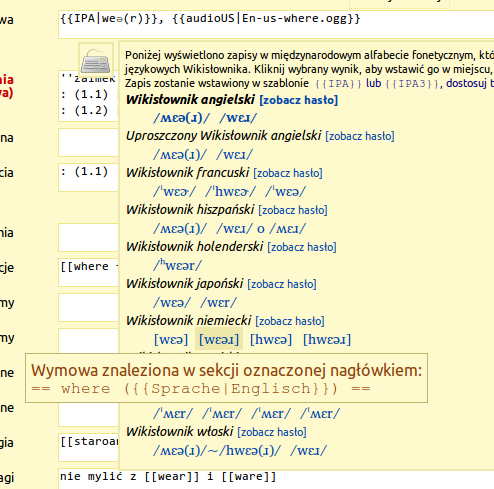
\includegraphics[width=0.65\textwidth]{iparesult}}
	\caption{Fragment okna wyświetlającego pobrane zapisy IPA}
	\label{fig:iparesult}
\end{illustration}

\subsubsection{Pobieranie grafik}
Innym elementem kopiowanym pomiędzy wersjami językowymi są ilustracje do haseł. Jest oczywiste, że ilustracja danego wyrazu będzie równie dobra w~każdej edycji Wikisłownika. Ponieważ znakomita większość używanych w~projektach Wikimedia grafik znajduje się na serwerach Wikimedia Commons (centralnego repozytorium plików dostępnych na wolnej licencji), a~w~polskich projektach tylko takie grafiki są używane, możliwe jest automatyczne odnajdywanie tych ilustracji.

\begin{opis}
\item[Projekty] Wikisłowniki odpowiadające sekcjom językowym w~haśle i~inne z~linków interwiki
\item[Zapytanie]
\begin{verbatim}
query = {
    titles: mw.config.get('wgTitle'),
    prop: 'revisions',
    rvprop: 'content'
};
\end{verbatim}
(Zawartość stron o~tytule równemu tytułowi obecnej strony)
\end{opis}

Skrypt odpowiadający za przetworzenie wyników zapytania działa dwuetapowo. Na początku z~obcojęzycznych haseł ekstrahowane są nazwy plików graficznych --- jest to dość proste do wykonania, ponieważ standardowy sposób wstawiania ich do haseł sprawia, że zawsze poprzedzone są dwukropkiem (alternatywnie mogą być parametrami szablonów, a~więc występować po znakach \kod@|@ lub \kod|=|), kończą się zaś oczywiście rozszerzeniem formatu graficznego. Już po odnalezieniu tych nazw możliwe byłoby zakończenie działania funkcji i~umożliwienie wprowadzenia redaktorowi pliku do polskiego hasła na podstawie jego nazwy. Aby jednak zwiększyć intuicyjność obsługi aplikacji i~wyświetlić użytkownikowi miniaturkę każdego z~plików, wykonywane jest kolejne zapytanie:

\begin{illustration}
	\fbox{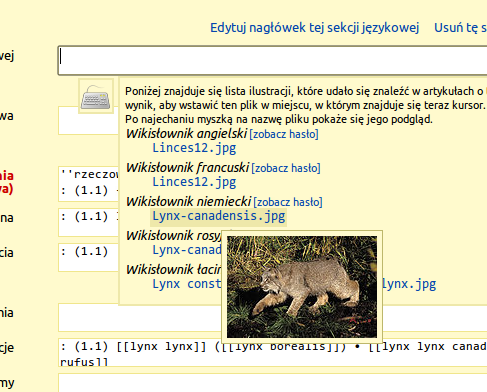
\includegraphics[width=0.65\textwidth]{picture}}
	\caption{Fragment okna do wyboru ilustracji wraz ze wskazaną miniaturą}
	\label{fig:pic}
\end{illustration}

\begin{opis}
\item[Projekty] Wikimedia Commons
\item[Zapytanie]
\begin{verbatim}
query = {
    titles: allImages.join('|'),
    prop: 'imageinfo',
    iiprop: 'url',
    iiurlwidth: 150,
    iiurlheight: 150
};
\end{verbatim}
(Adresy URL miniatur o~rozmiarach 150~\texttimes~150~px dla podanych plików)
\end{opis}

Lokalizacja miniatury ilustracji o~zadanej wielkości nie jest bezpośrednio zależna od nazwy pliku --- MediaWiki używa funkcji haszujących, aby umieścić ją w~jednym z~wielu katalogów. Dlatego zwykłymi metodami niezależnymi od MediaWiki nie jest możliwe natychmiastowe wyświetlenie ilustracji bez zapytania do API Wikimedia Commons, które przekaże niezbędne dane. Po otrzymaniu tej informacji aplikacja ładuje odpowiednie obrazy i~wyświetla je po najechaniu myszą na nazwę pliku, jak pokazano na ilustracji~\ref{fig:pic}.

\subsubsection{Pobieranie nagrań wymowy}
Aplikacja umożliwia także automatyczne odnajdywanie plików dźwiękowych z~wzorcową wymową danego słowa. Wyszukiwanie to odbywa się w~podobny sposób jak w~przypadku ilustracji --- tutaj kod haseł w~innych językach przeszukiwany jest na okoliczność wystąpienia nazwy pliku zakończonego na \kod|.ogg|. Zapytanie o~zawartość stron ma postać identyczną jak w~poprzednim przykładzie.

Nagrania wymowy, podobnie jak ilustracje, umieszczane są w~Wikimedia Commons. Dzięki zasadom obowiązujących w~tym projekcie nazwy tych plików są zestandaryzowane: mają postać \kod|<ISO>-<wyraz>.ogg| (np. \kod|De-Meerschweinchen.ogg| dla słowa \emph{Meerschweinchen} --- \emph{świnka morska}). Z~tego powodu możliwe jest dodatkowe wyszukanie pliku bezpośrednio w~zasobach Commons za pomocą API tego projektu. Dodatkowo dla słów angielskich i~niemieckich często pojawiają się warianty wymowy amerykańskiej, australijskiej czy austriackiej. Listing~\ref{code:audio} pokazuje, jak konstruowane jest zapytanie do Commons.

\begin{jscode}{code:audio}{Fragment funkcji \kod|EAutomator.getAudio|}
lang = $.ucFirst(EUtil.getActiveLangCode());
titles.push('File:' + lang + '-' + mw.config.get('wgTitle') + '.ogg');
if (lang === 'En') {
	titles.push('File:' + lang + '-uk-' + mw.config.get('wgTitle') + '.ogg');
	titles.push('File:' + lang + '-us-' + mw.config.get('wgTitle') + '.ogg');
	titles.push('File:' + lang + '-au-' + mw.config.get('wgTitle') + '.ogg');
}
if (lang === 'De') {
	titles.push('File:' + lang + '-at-' + mw.config.get('wgTitle') + '.ogg');
}

queries[EApi.commonsUrl()] = { titles: titles.join('|'), prop: 'info' };
\end{jscode}%$

\subsubsection{Pobieranie przykładów użycia}
Innym elementem procesu tworzenia lub edycji hasła w~Wikisłowniku jest podanie przykładu użycia --- pełnego zdania, w~którym występuje dany wyraz. Oczywiście to samo zdanie może nadawać się jako przykład użycia w~co najmniej kilku artykułach. Ponieważ wszystkie przykłady w~językach inny niż polski są dodatkowo tłumaczone (wersja polska pojawia się po znaku →), szczególnie wielu zdań można użyć ponownie w~przypadku słów polskich.

Pomocny okazuje się fakt, że wszystkie przykłady, a~także liczne inne elementy hasła, opatrywane są linkami do pojedynczych słów w~nich występujących. MediaWiki ma funkcję, która pozwala wykorzystać to do wspomagania edycji --- tzw. \emph{Linkujące}, czyli stronę specjalną podającą spis wszystkich stron z~linkami do podanej strony. Ponieważ w~analogiczną możliwość wyposażone jest API, można jednym zapytaniem pobrać zawartość kilkudziesięciu haseł, w~których występuje link do wybranego artykułu. Funkcja \kod|EParser.extractSubsections| (p.~listing~\ref{code:subs}) pozwala z~treści wszystkich tych haseł wybrać jedynie interesujące nas podsekcje --- w~tym przypadku są to \emph{przykłady}.

\begin{opis}
\item[Projekty] Polski Wikisłownik
\item[Zapytanie]
\begin{verbatim}
query = {
    generator: 'backlinks',
    gbltitle: mw.config.get('wgTitle'),
    gbllimit: 50,
    gblnamespace: 0,
    prop: 'revisions',
    rvprop: 'content'
};
\end{verbatim}
(Zawartość pierwszych 50~stron w~przestrzeni głównej, linkujących do obecnej strony)
\end{opis}

\begin{jscode}{code:subs}{Funkcja \kod|EParser.extractSubsections|}
extractSubsections : function (str, name) {
	var sec, index, re,
		sections = EParser.getSections(str),
		subsections = [];

	/* dla kazdej sekcji jezykowej w hasle */
	$.each(sections, function () {
		if (!this.content) {
			return true;
		}
		sec = this.content;
		/* wyszukanie pozycji szablonu podsekcji */
		index = sec.indexOf('{{' + name + '}}');
		if (index > -1) {
			sec = sec.substring(index + name.length + 4);
			/* wyszukanie kolejnej, dowolnej podsekcji i obciecie lancucha znakow */
			re = new RegExp('\\{\\{(' + EConstants.SUBSECTIONS.ALL.join('|') + ')[\\}\\|]');
			subsections.push(sec.substring(0, sec.search(re)));
		}
	});
	return subsections.join('');
}
\end{jscode}%$

Listing~\ref{code:example} przedstawia (nieco uproszczoną) funkcję odpowiadającą za wyłuskanie z~kodu stron linkujących do edytowanej możliwych przykładów użycia. Najważniejsze było tu skonstruowanie odpowiedniego wyrażenia regularnego (\kod|re|) i~odpowiednie zróżnicowanie wyrazów polskich i~niepolskich.

\begin{jscode}{code:example}{Funkcja \kod|EAutomator.getInternalExampleRe|}
getInternalExampleRe : function (result) {
	var examples = {},
		re = new RegExp("^:\\s*\\(\\d+\\.\\d+\\)\\s*('*[^\\n]*\\[\\[" +
			mw.config.get('wgTitle') + "[\\|\\]][^\\n]*)", 'm'),
		isPolish = EUtil.getActiveLangCode() === 'pl';

	/* na kazdej stronie linkujacej... */
	$.each(result[0].query.pages, function () {
		var content, ex;
		/* sprawdzamy tylko podsekcje z przykladami */
		content = EParser.extractSubsections(this.revisions[0]['*'], 'przyklady');
		if ((arr = re.exec(content)) !== null) {
			if (isPolish) {
				/* dla polskiego obcinamy czesc przed strzalka */
				ret = arr[1].replace(/(.*->\s*|''{1,2})/g, '');
				/* i sprawdzamy, czy nadal jest tam slowo */
				ex = re.exec(": (1.1) ''" + ret) === null ? null : ret;
			} else {
				/* dla innego tylko usuwamy pogrubienie tamtejszego slowa */
				ex = arr[1].replace(/''{1,2}/g, '');
			}
			if (ex) {
				examples[this.title] = $.trim(ex);
			}
		}
	});
	...
}
\end{jscode}

Przykładowe zdania odnalezione przez tę funkcję wstawiane są w~taki sam sposób jak inne automatycznie pobrane informacje. Przykładowy wynik działania skryptu zaprezentowany został na ilustracji~\ref{fig:example}.

\begin{illustration}
	\fbox{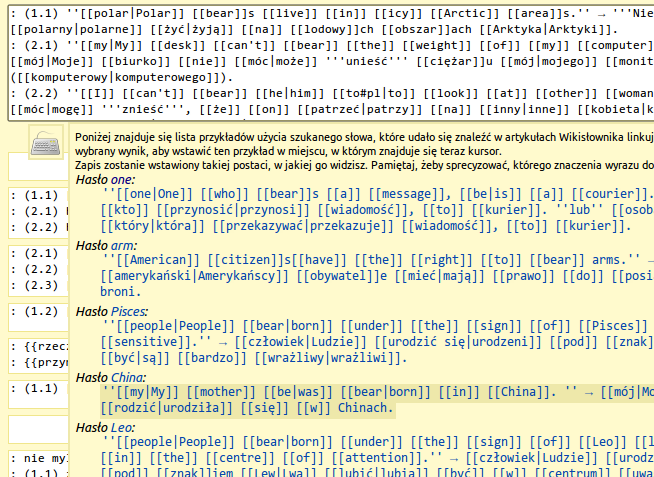
\includegraphics[width=\textwidth]{example}}
	\caption{Fragment okna wyświetlającego pobrane przykłady użycia}
	\label{fig:example}
\end{illustration}

W~projektach Wikimedia ważnym elementem edycji hasła jest uzupełnienie tzw. opisu zmian --- informacja o~tym, co zostało zmienione, widoczna jest np. w~historii zmian strony czy na specjalnych stronach z~ostatnimi zmianami lub stronami obserwowanymi przez użytkowników. Aby ułatwić redaktorowi edycję, pole to jest uzupełniane, jeśli wykonana zostanie jedna z~akcji opartych na pobieraniu informacji automatycznie z~innych stron. W~przypadku IPA i~przykładów użycia do opisu zmian dołączany jest link do strony, z~której pochodzi nowy element. W~ten sposób łatwiej jest prześledzić proces tworzenia hasła osobie z~zewnątrz.

\section{Wdrożenie i~dalszy rozwój}
\label{sec:impl-deploy}


%licencja
%IE < Win7 :(


\chapter{Podsumowanie}
Celem niniejszej pracy było przedstawienie aplikacji, która ma za zadanie znacząco uprościć edycję haseł w~Wikisłowniku. Wydaje się, że w~bliskiej przyszłości potwierdzi się, że projekt ten zakończył się sukcesem. Wprawdzie często w~projektach Fundacji Wikimedia nowe funkcje wprowadzane są bardzo powoli, jednak jak wielokrotnie wspomniano, specyfika  polskiego Wikisłownika odróżnia go od innych przedsięwzięć takich jak Wikipedia. Opisana aplikacja jest całkowicie niezależna od innych rozwiązań technologicznych przeznaczonych dla serwisów opartych na MediaWiki, a~jej przyszłość zależy praktycznie wyłącznie od stosunkowo jednomyślnej społeczności, traktującej nowy formularz edycyjny z~zadowoleniem, a~nawet entuzjazmem.

Co ważne, nowy formularz powstał praktycznie od zera, co było możliwe dzięki efektywnemu wykorzystaniu jQuery --- bez użycia tego typu biblioteki stworzenie zaawansowanego programu byłoby znacznie bardziej złożone. W~trakcie implementacji konieczne było rozwiązanie wielu problemów, które oczywiście nie mogły wszystkie zostać opisane w~niniejszej pracy dość wyczerpująco. Wprowadzenie aplikacji jako standardu w~Wikisłowniku powinno pozytywnie wpłynąć na rozwój tego projektu. Funkcje przetwarzające wikitekst zostały starannie przygotowane i~przetestowane we współpracy z~aktywnymi redaktorami, co pozwoli na dalsze ujednolicenie kodu artykułów --- na czym z~pewnością skorzystają kolejne projekty programistyczne w~Wikisłowniku.

Tworzenie tego typu aplikacji było ciekawym wyzwaniem, odmiennym od znakomitej większości projektów informatycznych. Dzięki otwartemu charakterowi aplikacja ma szansę okazać się przydatna dla tysięcy osób, które chciałyby wspomóc jeden z~najlepiej rozwiniętych polskich projektów opartych na koncepcji wiki. Kolejne miesiące prawdopodobnie przyniosą dalszy rozwój aplikacji --- podstawowy etap został zakończony, ale widoki na przyszłość prezentują się ciekawie. Szczególnie warte uwagi jest, że można liczyć na kolejne zastosowania modułu umożliwiającego wygodną automatyzację edycji na bazie API. W~polskich projektach Wikimedia jest to pierwsza aplikacja, która intensywnie korzysta z~tego interfejsu i~w~takim stopniu pozwala na uproszczenie procesu edycji artykułów, niekiedy rzeczywiście żmudnego. Skorzystają na tym zarówno doświadczeni użytkownicy, mający na koncie tysiące stworzonych haseł, jak i~nowicjusze, których nie przerazi już widok, który ujrzą po kliknięciu w~zakładkę ,,edytuj''.


\appendix
\chapter{Zawartość płyty CD}
\begin{enumerate}
\item Niniejsza praca:
	\begin{itemize}
	\item w~formacie PDF,
	\item kod źródłowy \XeTeX,
	\end{itemize}
\item Kod źródłowy aplikacji:
	\begin{itemize}
	\item w~postaci modułowej,
	\item w~postaci złączonej do jednego pliku,
	\end{itemize}
\item Skrypt do łączenia aplikacji w~jeden plik.
\end{enumerate}


\chapter{Podsekcje występujące w~hasłach Wikisłownika}
\label{wikt:subsections}
\begin{opis}
	\item[Szablon] \verb|{{zapis hieroglificzny}}|
	\item[Zawartość] Zapis hieroglificzny słowa w~języku staroegipskim, pokazany za~pomocą grafik PNG z~repozytorium Wikimedia Commons. Oznaczenie \kod|(1.1)| odnosi się do numeracji w~sekcji \emph{znaczenia}.
	\item[Języki] tylko staroegipski\footnote{Rubryka \emph{Języki} precyzuje, w~których sekcjach językowych występuje dana podsekcja. Oprócz zwykłych sekcji, odpowiadających danemu językowi, istnieją także nietypowe: \emph{użycie słowa obcego w~języku polskim} i~\emph{znak chiński}}.
	\item[Przykład]
		\begin{verbatim}
			{{zapis hieroglificzny}}
			: (1.1) [[Plik:Egyptian-Pr-cnḫ.PNG]];
			[[Plik:Egyptian-Pr-cnḫ2.PNG]];
			[[Plik:Egyptian-Pr-cnḫ3.PNG]]
		\end{verbatim}
\end{opis}
\spacer
\begin{opis}
	\item[Szablon] \verb|{{ortografie}}|
	\item[Zawartość] Inne sposoby zapisu tytułu hasła. Zazwyczaj chodzi o~alternatywną pisownię w~języku, do zapisu którego używane są dwa alfabety (np.\ serbski). Do prezentacji pisowni mogą być używane szablony wyświetlające dodatkowe informacje.
	\item[Języki] azerski, białoruski, dżuhuri, gagauski, krymskotatarski, ladino, mołdawski, serbski, slovio, tatarski, turkmeński, ujgurski
	\item[Przykład]
		\begin{verbatim}
			{{ortografie}} Мацедониа
		\end{verbatim}
\end{opis}
\spacer
\begin{opis}
	\item[Szablon] \verb|{{transliteracja}}|
	\item[Zawartość] Transliteracja słowa zapisanego w~obcym alfabecie na alfabet łaciński. \\ W~przeciwieństwie do transkrypcji transliteracja może być wykonywana automatycznie --- każda litera alfabetu obcego konwertowana jest na jeden lub więcej znaków w~alfabecie łacińskim. Obecnie często używany jest szablon \kod|{{translit}}|, który umożliwia automatyczną konwersję za pomocą JavaScriptu niektórych alfabetów podczas odczytywania strony.
	\item[Języki] abazyński, abchaski, adygejski, akadyjski, amharski, arabski, aramejski, assamski, awarski, baszkirski, beludżi, bengali, birmański, bułgarski, chakaski, czeczeński, czuwaski, dzongkha, erzja, gocki, gruziński, gudźarati, gyyz, hebrajski, hindi, inguski, inuktitut, jidysz, kannada, kaszmirski, kazachski, khmerski, kirgiski, komi, komi\dywiz{}jaźwiński, kri, kurdyjski, laotański, lezgiński, macedoński, malajalam, malediwski, marathi, maryjski, mongolski, nepalski, newarski, nowogrecki, orija, ormiański, osetyjski, paszto, pendżabski, perski, romski, rosyjski, sanskryt, sindhi, sorani, staro\dywiz{}cerkiewno\dywiz{}słowiański, starogrecki, staroormiański, sumeryjski, syngaleski, tabasarański, tadżycki, tajski, tamazight, tamilski, telugu, tybetański, ukraiński, urdu, zarfatit
	\item[Przykład]
		\begin{verbatim}
			{{transliteracja}} Moskva
		\end{verbatim}
\end{opis}
\spacer
\begin{opis}
	\item[Szablon] \verb|{{transkrypcja}}|
	\item[Zawartość] Transkrypcja słowa zapisanego w~obcym alfabecie na język polski, czyli przedstawienie go w~formie dającej informacje o~rzeczywistej wymowie
	\item[Języki] standardowo tylko staroegipski, podsekcja ta może być jednak dodawana w~wielu innych językach (przykład w~jidysz)
	\item[Przykład]
		\begin{verbatim}
			{{transkrypcja}}
			: (1.1-3) {{YIVO|{{lp}} khaver {{lm}} khaveyrim}}; polska: {{lp}}
			chawer {{lm}} chawejrim
			: (1.4) {{YIVO|{{lp}} khover {{lm}} khovers}}; polska: {{lp}}
			chower; {{lm}} chowers
		\end{verbatim}
\end{opis}
\spacer %http://pl.wiktionary.org/wiki/Kategoria:Szablony_szablon%C3%B3w_hase%C5%82
\begin{opis}
	\item[Szablon] \verb|{{czytania}}|
	\item[Zawartość] Wyjaśnienie możliwego wymawiania znaków kanji używanych w~języku japońskim. Występują dwa sposoby czytania: on'yomi i~kun'yomi. Do ich prezentacji używane są szablony \kod|{{on}}| i~\kod|{{kun}}|.
	\item[Języki] tylko japoński
	\item[Przykład]
		\begin{verbatim}
			{{czytania}} {{on}} ビ (bi); {{kun}} はな (hana)
		\end{verbatim}
\end{opis}
\spacer
\begin{opis}
	\item[Szablon] \verb|{{klucz}}|
	\item[Zawartość] Elementy, według których układane są słowniki języka chińskiego.
	\item[Języki] tylko znak chiński
	\item[Przykład]
		\begin{verbatim}
			{{klucz}} 157 足 + 6
		\end{verbatim}
\end{opis}
\spacer
\begin{opis}
	\item[Szablon] \verb|{{kreski}}|
	\item[Zawartość] Liczba kresek użytych do napisania danego znaku. Informacja służy m.in.\ do ułatwienia odnajdywania znaków w~papierowych słownikach.
	\item[Języki] znak chiński, koreański
	\item[Przykład]
		\begin{verbatim}
			{{kreski}} 13
		\end{verbatim}
\end{opis}
\spacer
\begin{opis}
	\item[Szablon] \verb|{{warianty}}|
	\item[Zawartość] Szablon powiększający znak chiński i~ewentualnie jego warianty. Szablon ten jest używany inaczej niż większość: nie odpowiada jedynie za wyświetlenie nagłówka, a~zawartość sekcji wstawiana jest jako parametr. Najczęściej w~parametrze pojawia się szablon \kod|{{zch-w}}|, odpowiadający za prezentację znaku.
	\item[Języki] tylko znak chiński
	\item[Przykład]
		\begin{verbatim}
			{{warianty|{{zch-w}}}}
		\end{verbatim}
\end{opis}
\spacer
\begin{opis}
	\item[Szablon] \verb|{{kolejność}}|
	\item[Zawartość] Kolejność stawiania kresek w~znaku chińskim, ilustrowana za pomocą grafiki dostępnej w~projekcie Wikimedia Commons. W~tej podsekcji używane są szablony \kod|{{zch-komiks}}|, \kod|{{zch-cienie}}| i~\kod|{{zch-animacja}}|, które ładują automatycznie grafiki o~nazwie odpowiadającej hasłu, jeśli te istnieją.
	\item[Języki] tylko znak chiński
	\item[Przykład]
		\begin{verbatim}
		{{kolejność}}
		{{zch-komiks}}
		\end{verbatim}
\end{opis}
\spacer
\begin{opis}
	\item[Szablon] \verb|{{wymowa}}|
	\item[Zawartość] Jedna z~kluczowych podsekcji we~wszystkich językach. Podawane są w~niej informacje na temat wymowy danego hasła, zarówno za pomocą alfabetów fonetycznych (jak np.\ IPA oraz alfabet słowiański), jak i~nagrań dźwiękowych umieszczonych w~Wikimedia Commons. Do opisywania wymowy stosowane są szablony \kod|{{IPA}}|, \kod|{{IPA2}}|, \kod|{{IPA3}}|, \kod|{{IPA4}}|. Wymowa słów polskich dodawana jest automatycznie przez bota uruchomionego przez jednego z~administratorów Wikisłownika. Bot ten jest skomplikowanym programem napisanym w~Javie~\cite{wikt:olafbot}, generującym wymowę na podstawie publikacji Danuty Ostaszewskiej i~Jolanty Tambor~\cite{fonetyka}.
	Pliki dźwiękowe dodawane są szablonem \kod|{{audio}}|.
	\item[Języki] wszystkie poza znakiem chińskim i~użyciem międzynarodowym
	\item[Przykład]
		\begin{verbatim}
		{{wymowa}} {{audio|Pl-samochód.ogg}}, {{IPA3|sãˈmɔxut}},
		{{AS3|sãm'''o'''χut}}, {{objaśnienie wymowy|WYG|NAZAL}}
		\end{verbatim}
\end{opis}
\spacer
\begin{opis}
	\item[Szablon] \verb|{{znaczenia}}|
	\item[Zawartość] Jedyna podsekcja obowiązkowa, w~której podawane jest znaczenie hasła. Zawartość podsekcji dzielona jest najpierw na części mowy, potem na poszczególne znaczenia, które zostają ponumerowane zgodnie z~obowiązującym schematem. W~hasłach polskich podawane jest dłuższe znaczenie, w~innych językach tłumaczenie na polski. Znaczenia te są linkami do objaśnień form podstawowych poszczególnych słów --- linkowanie to stanowi dość duże utrudnienie przy tworzeniu hasła.
	\item[Języki] wszystkie
	\item[Przykłady] Hasło angielskie:
		\begin{verbatim}
		{{znaczenia}}
		''rzeczownik''
		: (1.1) [[zamówienie]]
		: (1.2) [[rozkaz]]
		: (1.3) [[porządek]]
		: (1.4) {{syst}} [[rząd]]
		: (1.5) {{mat}} [[rząd]]
		''czasownik''
		: (2.1) [[zamawiać]]
		: (2.2) [[rozkazywać]]
		\end{verbatim}
		Hasło polskie:
		\begin{verbatim}
		{{znaczenia}}
		''rzeczownik, rodzaj męski''
		: (1.1) [[budynek]] [[warowny]]; {{wikipedia|zamek (architektura)}}
		: (1.2) [[mechanizm]] [[zamykać|zamykający]] [[drzwi]],
		[[szuflada|szuflady]]; {{wikipedia|zamek (urządzenie)}}
		: (1.3) [[zapięcie]] [[garderoba|garderoby]],
		{{zob|[[zamek błyskawiczny]]}}.
		: (1.4) [[element]] [[składowy]] [[broń|broni]] [[palny|palnej]];
		{{wikipedia|zamek (broń)}}
		\end{verbatim}
\end{opis}
\spacer
\begin{opis}
	\item[Szablon] \verb|{{determinatywy}}|
	\item[Zawartość] Znak określający, o~jaką klasę znaczeniową wyrazów chodzi w~danym haśle. Wyświetlana jest grafika z~Wikimedia Commons.
	\item[Języki] tylko staroegipski
	\item[Przykład]
		\begin{verbatim}
			{{determinatywy}}
			: (1.1) [[Plik:Egyptian-nb ʿnḫ-determinative.PNG]]
		\end{verbatim}
\end{opis}
\spacer
\begin{opis}
	\item[Szablon] \verb|{{odmiana}}|
	\item[Zawartość] Odmiana wyrazu, prezentowana na różne sposoby. Występują np.\ szablony, które generują odmianę na podstawie formy podstawowej hasła. Niekiedy podawana jest jedynie deklinacja lub koniugacja (z~odnośnikiem do tabel ją przedstawiających), gdzie indziej cała odmiana.
	\item[Języki] wszystkie poza znakiem chińskim
	\item[Przykład]
		\begin{verbatim}
			{{odmiana}}
			: (1.1-2) читать {{ter}} {{lp}} читаю, читаешь, читает; {{lm}} читаем,
			читаете, читают; {{przesz}} {{lp}} читал / читала / читало; {{lm}} читали;
			{{rozk}} {{lp}} читай; {{ims}} читающий; читаемый; читая
		\end{verbatim}
\end{opis}
\spacer
\begin{opis}
	\item[Szablon] \verb|{{przykłady}}|
	\item[Zawartość] Przykłady użycia danego słowa w~zdaniu. W~przypadku języków innych niż polski tłumaczenie przykładu podane jest po znaku →. Podobnie jak znaczenia, przykłady są linkowane.
	\item[Języki] wszystkie poza znakiem chińskim
	\item[Przykład]
		\begin{verbatim}
			{{przykłady}}
			: (2.1) ''[[Michael]] '''locks''' [[his]] [[house]] [[every]]
			[[day]]. '' → [[Michał]] [[codziennie]] '''[[zamykać|zamyka]]''' [[swój]]
			[[dom]] (na klucz).
		\end{verbatim}
\end{opis}
\spacer
\begin{opis}
	\item[Szablon] \verb|{{składnia}}|
	\item[Zawartość] Podsekcja zawiera informacje o~używaniu słowa w~połączeniu z~przyimkami czy przypadkami.
	\item[Języki] wszystkie poza znakiem chińskim
	\item[Przykład]
		\begin{verbatim}
			{{składnia}}
			: (1.2) jechać +{{N}}; jechać [[do]] +{{D}}, jechać [[na]] +{{B}}
		\end{verbatim}
\end{opis}
\spacer
\begin{opis}
	\item[Szablon] \verb|{{kolokacje}}|
	\item[Zawartość] Kolokacje to często używane zestawienia słów, w~których (w~przeciwieństwie do związków frazeologicznych) znaczenie całości wynika ze znaczenia poszczególnych wyrazów.
	\item[Języki] wszystkie poza znakiem chińskim
	\item[Przykład]
		\begin{verbatim}
			{{kolokacje}} [[mieć]] / [[budzić]] / [[odbierać]] nadzieję • [[promyk]]
			nadziei • [[ziścić]] nadzieje • [[karmić]] [[się]] nadzieją
		\end{verbatim}
\end{opis}
\spacer
\begin{opis}
	\item[Szablon] \verb|{{synonimy}}|
	\item[Zawartość] Wyrazy bliskoznaczne, synonimy.
	\item[Języki] wszystkie poza znakiem chińskim
	\item[Przykład]
		\begin{verbatim}
			{{synonimy}}
			: (1.1) [[ufność]], [[wiara]], [[zawierzenie]], [[pociecha]]
		\end{verbatim}
\end{opis}
\spacer
\begin{opis}
	\item[Szablon] \verb|{{antonimy}}|
	\item[Zawartość] Wyrazy przeciwstawne, antonimy
	\item[Języki] wszystkie poza znakiem chińskim
	\item[Przykład]
		\begin{verbatim}
			{{antonimy}}
			: (1.1) [[rezygnacja]], [[zwątpienie]], [[beznadzieja]]
		\end{verbatim}
\end{opis}
\spacer
\begin{opis}
	\item[Szablon] \verb|{{złożenia}}|
	\item[Zawartość] W~językach japońskim i~koreańskim podsekcja ta podaje słowa, które powstają jako złożenie danego hasła z~innym. Użyty w~przykładzie szablon \kod|{{furi}}| pomaga dobrze wyświetlić furiganę --- japońskie pismo.
	\item[Języki] koreański i~japoński
	\item[Przykład]
		\begin{verbatim}
			{{złożenia}} {{furi|五日|いつか}}, {{furi|五月|ごがつ}},
			{{furi|五輪|ごりん}}, {{furi|五輪大会|ごりんたいかい}}
		\end{verbatim}
\end{opis}
\spacer
\begin{opis}
	\item[Szablon] \verb|{{pokrewne}}|
	\item[Zawartość] Wyrazy pokrewne do danego wyrazu podstawowego. W~przypadku większej grupy wyrazów wspólnej dla wielu haseł może wystąpić odsyłacz do wyrazu podstawowego, np. w~haśle \emph{kocur}: \kod@{{zob|[[kot]]}}@.
	\item[Języki] wszystkie poza znakiem chińskim
	\item[Przykład]
		\begin{verbatim}
			{{pokrewne}}
			: (1.1) {{rzecz}} [[picklock]], [[locksmith]], [[locknut]]
			: (1.2) {{rzecz}} [[dreadlock]]
			: (1.3) {{rzecz}} [[airlock]], [[lockage]]
			: (2.1) {{przym}} [[lockable]]; {{rzecz}} [[locker]]
		\end{verbatim}
\end{opis}
\spacer
\begin{opis}
	\item[Szablon] \verb|{{pochodne}}|
	\item[Zawartość] Odpowiednik podsekcji \emph{pokrewne} dla morfemów w~esperanto, stanowiących osobne hasła.
	\item[Języki] esperanto
	\item[Przykład]
		\begin{verbatim}
			{{pochodne}} {{rzecz}} [[zebro]], [[zebrino]], [[zebrido]]
		\end{verbatim}
\end{opis}
\spacer
\begin{opis}
	\item[Szablon] \verb|{{frazeologia}}|
	\item[Zawartość] Podsekcja zawiera związki frazeologiczne, które prezentowane są podobnie jak kolokacje. Różnica między kolokacjami a~związkami frazeologicznymi polega na tym, że w~przypadku tych drugich znaczenie związku nie wynika bezpośrednio ze znaczeń poszczególnych wyrazów.
	\item[Języki] wszystkie poza znakiem chińskim
	\item[Przykład]
		\begin{verbatim}
			{{frazeologia}}
			: [[psi urok]] • [[tu leży pies pogrzebany]] • {{wulg}} [[pies kogoś
			jebał]] • [[pies ogrodnika]] • {{pot}} [[pies na baby]] • [[pogoda pod
			psem]] • [[psu na budę]] • [[pieskie życie]] • [[psia wachta]] • [[psia
			koja]] • [[pies Pawłowa]] • [[nie dla psa kiełbasa]] • [[pies łańcuchowy
			Darwina]] • [[na psa urok]] • [[ni pies, ni wydra]] • [[schodzić na
			psy]] • [[łgać jak pies]] • [[delikatny jak francuski piesek]] •
			[[francuski piesek]] • [[pies z nim tańcował]] • [[psi żywot]] • [[psie
			figle]] • [[psi obowiązek]] • [[całować psa w nos]] ...
			: zobacz też: [[Aneks:Przysłowia polskie - zwierzęta#pies|przysłowia o
			psie]]
		\end{verbatim}
\end{opis}
\spacer
\begin{opis}
	\item[Szablon] \verb|{{etymologia}}|
	\item[Zawartość] Pochodzenie wyrazu, zapisywane za pomocą szablonów \kod|{{etym}}| i~\kod|{{etymn}}|.
	\item[Języki] wszystkie
	\item[Przykład]
		\begin{verbatim}
			{{etymologia}}
			: {{etym|prasłowiański|*ne}} < {{etym|praindoeuropejski|*ne}} 'nie'
			: {{por}} {{etymn|czeski|ne}}, {{etymn|rosyjski|не}},
			{{etymn|litewski|ne}}, {{etymn|łaciński|ne}}
		\end{verbatim}
\end{opis}
\spacer
\begin{opis}
	\item[Szablon] \verb|{{kody}}|
	\item[Zawartość] Informacje na temat wprowadzania znaków chińskich za pomocą klawiatury w~różnych metodach oraz kodowania Unicode. Podobnie jak w~przypadku podsekcji \emph{warianty}, i~tutaj szablon przyjmuje parametry pozwalające na zestandaryzowane wyświetlanie.
	\item[Języki] tylko znak chiński
	\item[Przykład]
		\begin{verbatim}
			{{kody |cjz=田金 |cjl=WC |cr=6021<sub>0</sub> |u=56db}}
		\end{verbatim}
\end{opis}
\spacer
\begin{opis}
	\item[Szablon] \verb|{{hanja}}|
	\item[Zawartość] W~tej podsekcji podawana jest pisownia danego słowa koreańskiego w~piśmie hanja (hancha), czyli pisownia zapożyczona z~języka chińskiego. Częściej w~koreańskim używany jest alfabet hangul.
	\item[Języki] tylko koreański
	\item[Przykład]
		\begin{verbatim}
			{{hanja}} [[憲法]]
		\end{verbatim}
\end{opis}
\spacer
\begin{opis}
	\item[Szablon] \verb|{{słowniki}}|
	\item[Zawartość] Informacja na temat występowania danego znaku chińskiego w~słownikach KangXi, Dai Kanwa Jiten, Dae Jaweon i~Hanyu Da Zidian.
	\item[Języki] tylko znak chiński
	\item[Przykład]
		\begin{verbatim}
			{{słowniki|kx=1163.080|dkj=35533|dj=1628.020|hdz=63974.090}}
		\end{verbatim}
\end{opis}
\spacer
\begin{opis}
	\item[Szablon] \verb|{{uwagi}}|
	\item[Zawartość] Dodatkowe informacje, np.\ częste błędy, odpowiedzi na typowe wątpliwości.
	\item[Języki] wszystkie
	\item[Przykład]
		\begin{verbatim}
			{{uwagi}}
			: (1.1) forma ''tylni'' dla przymiotnika rodzaju męskiego w liczbie
			pojedynczej jest błędna, może odnosić się ona jedynie do liczby mnogiej
			<ref>{{PoradniaPWN|id=9687|hasło=tylny czy tylni?}}</ref>
		\end{verbatim}
\end{opis}
\spacer
\begin{opis}
	\item[Szablon] \verb|{{tłumaczenia}}|
	\item[Zawartość] Podsekcja ta pełni funkcję słownika z~języka polskiego na inne. Podawane są odnośniki do wyrazów będących tłumaczeniami danego słowa polskiego.
	\item[Języki] tylko polski
	\item[Przykład]
		\begin{verbatim}
			{{tłumaczenia}}
			* angielski: (1.1) [[date]], [[appointment]]
			* arabski: (1.1) [[تعيين]]
			* francuski: (1.1) [[rendez-vous]]
			* rosyjski: (1.1) [[свидание]], {{pot}} [[свиданка]]
			* szwedzki: (1.1) [[träff]] {{w}}
		\end{verbatim}
\end{opis}
\spacer
\begin{opis}
	\item[Szablon] \verb|{{źródła}}|
	\item[Zawartość] Źródła dla informacji podanych w~haśle. Zazwyczaj sekcja ta składa się ze znacznika \kod|<references/>|, który powoduje wyświetlenie w~tym miejscu przypisów wstawionych w~poprzedzającej zawartości strony znaczników \kod|<ref>...</ref>|.
	\item[Języki] wszystkie
	\item[Przykład]
		\begin{verbatim}
			{{źródła}}
			<references/>
		\end{verbatim}
\end{opis}


\appendix

\cleardoublepage
\addcontentsline{toc}{chapter}{Bibliografia}
\bibliographystyle{plunsrt}
\bibliography{mgr}

\newpage
\addcontentsline{toc}{chapter}{Spis ilustracji}
\listoffigures
\addcontentsline{toc}{chapter}{Spis tabel}
\listoftables
\addcontentsline{toc}{chapter}{Spis listingów}
\lstlistoflistings
\end{document}

